% Complete text source. Compile from the package root with figures/.
\documentclass[11pt,a4paper]{article}
\usepackage[T1]{fontenc}
\usepackage[utf8]{inputenc}
\usepackage{lmodern}
\usepackage[margin=25mm,headheight=15pt]{geometry}
\usepackage{amsmath,amssymb,amsthm,mathtools}
\usepackage{microtype}
\usepackage{graphicx,booktabs,longtable,array,enumitem}
\usepackage{xcolor,xurl,hyperref,fancyhdr}
\definecolor{inkblue}{HTML}{173D63}
\definecolor{muted}{HTML}{555C65}
\hypersetup{colorlinks=true,linkcolor=inkblue,citecolor=inkblue,urlcolor=inkblue,
  pdftitle={Sharp Gaussian Bounds, Cyclic Distribution Torsion, and Extremal Lerch Zeros},
  pdfauthor={Research continuation prepared for the ProveIt project}}
\urlstyle{same}
\pagestyle{fancy}
\fancyhf{}
\fancyhead[L]{\small\color{muted}ProveIt research continuation}
\fancyhead[R]{\small\color{muted}10 October 2026}
\fancyfoot[C]{\thepage}
\renewcommand{\headrulewidth}{0.25pt}
\setlength{\parskip}{3.5pt}
\setlength{\parindent}{1.1em}
\setlength{\emergencystretch}{2em}
\setcounter{tocdepth}{2}
\numberwithin{equation}{section}
\newtheorem{theorem}{Theorem}[section]
\newtheorem{lemma}[theorem]{Lemma}
\newtheorem{proposition}[theorem]{Proposition}
\newtheorem{corollary}[theorem]{Corollary}
\theoremstyle{definition}
\newtheorem{definition}[theorem]{Definition}
\newtheorem{conjecture}[theorem]{Conjecture}
\newtheorem{example}[theorem]{Example}
\theoremstyle{remark}
\newtheorem{remark}[theorem]{Remark}
\DeclareMathOperator{\Li}{Li}
\DeclareMathOperator{\sech}{sech}
\DeclareMathOperator{\ord}{ord}
\renewcommand{\Im}{\operatorname{Im}}
\renewcommand{\Re}{\operatorname{Re}}
\newcommand{\snapshot}{\texttt{a0a90ef31877f98be437191c48b46f02d5456867}}
\setlist{itemsep=3pt,topsep=5pt}
\newcolumntype{L}[1]{>{\raggedright\arraybackslash}p{#1}}
\begin{document}
\hypersetup{pageanchor=false}
\begin{titlepage}
\centering
{\large\color{inkblue}ANALYSIS / POLYLOGARITHMS\par}
\vspace{20mm}
{\LARGE\bfseries Sharp Gaussian Bounds,\\[5pt]
Cyclic Distribution Torsion,\\[5pt]
and Extremal Lerch Zeros\par}
\vspace{8mm}
{\large Critical Euler constants, exact inverse expansions,\\
finite jets, and a certified reduction obstruction\par}
\vspace{12mm}
{\large A research continuation prepared for the ProveIt project\par}
\vspace{3mm}
{10 October 2026\par}
\vspace{12mm}
\begin{minipage}{0.91\textwidth}
\small
\textbf{Abstract.}
We continue the manuscript and incoming reports in a fixed ProveIt
snapshot. A beta-mixture representation proves strict monotonicity of
$-\Im\Li_{a,w-a}(i,1)$ in the outer order for every positive total
order $w$. This settles the incoming sharp critical Euler conjecture:
the best uniform constant is $\pi/4+(\log2)/2$. The sharp Gaussian
envelope $C(w)=\beta(w)+2^{-w}\eta(w)$ has a unique nondegenerate
maximum, certified at $w=1.30221658710124\ldots$, with value
$1.13656110333950\ldots$. We prove strict normalized Mellin
log-concavity, explicit endpoint identities, Turan inequalities, and
an all-order inverse generalized-power expansion with a closed
coefficient formula. A positive secant identity represents every
Euler remainder for all positive real orders, and proves absolute
Euler convergence even below the signed-measure threshold.

For weighted distributions on a finite cyclotomic grid, we calculate
coinvariants under a prime-order symmetry with a split fixed factor.
The complete integral torsion and all one-variable finite jets are
governed by a multiplicative character compatibility condition. For
the Stieltjes--Lerch derivative family, a finite resolvent identity
moves the largest positive zero strictly left even without saturation.
At index two we prove a global lower-branch dichotomy and an exact
endpoint criterion; certified signs give a unique minimum at derivative
order two and strict decrease of both branches at order three.
Finally, an integer functional separates the still-conjectural $S_6$
target from an enlarged, precisely specified family of 5,131 relations.
Analytic proofs, exact replay programs, diagnostic calculations,
source provenance, editorial proposals, and further research questions
are supplied together.
\end{minipage}
\vfill
\begin{minipage}{0.91\textwidth}
\small\color{muted}
Baseline commit: \snapshot.\\
Theorems are proved in ordinary mathematics, with exact computation
where explicitly indicated. This document is a research contribution
for review and integration, not a claim of completed proof-assistant
formalization or an exhaustive priority search.
\end{minipage}
\end{titlepage}
\pagenumbering{roman}
\hypersetup{pageanchor=true}
\begingroup
\small
\setlength{\parskip}{0pt}
\tableofcontents
\endgroup
\clearpage
\pagenumbering{arabic}
% BEGIN included source: article/introduction.tex
\section{Research baseline and contribution map}
\label{sec:introduction}

The manuscript is a developing research corpus, with newer incoming
reports that sometimes settle questions still listed as open elsewhere.
A continuation must reconcile that history before selecting targets.
We therefore use a single pinned version of Vladimir Reshetnikov's
ProveIt repository \cite{repo}: commit \snapshot, dated 10 October 2026
UTC. The inspection covered the manuscript's 40 chapter source files,
its editorial and validation material, and all 16 archives present in
\path{docs/incoming}. The 65 retrieved source objects, including those
archives, have paths, byte counts, and SHA-256 hashes in the accompanying
provenance manifest. This is a source and dependency audit of the present
continuation, not an assertion that every proof in the entire corpus
has been reverified.

The most useful unresolved targets lie at the intersection of positive
integral representations, exact formal relations, and zero geometry.
The work below develops all three. Its principal resolved conjecture is
the sharp critical constant in the real-order report \cite{realorder}.
The prime-order distribution calculation answers a proposed extension
of reflection torsion \cite{integraljets}. The Lerch results extend the
branch analysis beyond the cases already proved in the incoming
boundary and global-phase reports \cite{lershape:Boundary,lershape:Globalphase}.
The $S_6$ computation gives a rigorous limitation of a larger finite
proof search, while leaving the numerical identity open.

\subsection{Conventions and distinctions}

We use decreasing-index multiple polylogarithms:
\[
 \Li_{s_1,\ldots,s_d}(z_1,\ldots,z_d)
 =\sum_{n_1>\cdots>n_d>0}
   \frac{z_1^{n_1}\cdots z_d^{n_d}}
        {n_1^{s_1}\cdots n_d^{s_d}},
\]
initially in a domain of convergence. In particular
$F_{a,b}(z)=\Li_{a,b}(z,1)$ and $g_{a,b}=\Im F_{a,b}(i)$.
The positive real orders $a,b$ need not be integers. At boundary points
we specify analytic or Abel values when the ordinary series diverges.
We write $\beta(s)=\sum_{j\ge0}(-1)^j(2j+1)^{-s}$ and
$\eta(s)=\sum_{j\ge1}(-1)^{j-1}j^{-s}$ where their series converge,
and use their analytic continuations elsewhere. Standard conventions
are also recorded in the DLMF \cite{dlmf-polylog,dlmf-hurwitz}.

There are two different weights in this article: $a+b$ is the total
order of a Gaussian double polylogarithm, whereas the integer coefficients
$a_p$ in a distribution relation are arbitrary formal parameters.
The parameters $n,k,\rho$ in the Lerch family denote Stieltjes index,
derivative order, and deformation parameter. They are introduced afresh
in Section~\ref{lershape:sec:main}.

An equality of complex periods, membership in a specified rational
relation span, and a Smith invariant of an integral formal module are
different assertions. Our notation and proofs retain those distinctions.
In particular, the torsion theorem does not claim torsion among complex
numbers, and the $S_6$ separator does not claim numerical independence.

\subsection{What is added to the inspected baseline}

\begin{table}[htbp]
\centering
\begin{tabular}{@{}L{0.21\textwidth}L{0.39\textwidth}L{0.33\textwidth}@{}}
\toprule
Topic & Result in this continuation & Scope and proof status\\
\midrule
Critical Gaussian values & Strict allocation monotonicity for every
positive total order; sharp Euler constant on $a+b=1$
& Analytic proofs; resolves the incoming critical conjecture.\\[5pt]
Global envelope & A unique maximum of $\beta(w)+2^{-w}\eta(w)$,
sharp bound for all positive Gaussian orders, and inverse coefficients
& Analytic shape theorem plus rational maximum enclosure.\\[5pt]
Euler remainders & A positive secant integral and an exact example of
increasing normalized errors off the critical line
& Analytic identities; prevents an unsupported extension in $N$.\\[5pt]
Cyclic distributions & Integral coinvariants and all one-variable
finite jets for a split prime-order action
& Complete formula under explicit arithmetic hypotheses.\\[5pt]
Lerch zeros & Finite extremal-zero comparison; lower-branch dichotomy;
order-two minimum and order-three decrease
& Analytic theorems with exact endpoint sign certificates.\\[5pt]
Weight-seven reduction & Separation of the $S_6$ target from 5,131
specified relations through depth four
& Integer certificate; the period identity remains conjectural.\\
\bottomrule
\end{tabular}
\end{table}

The beta allocation identity is the main analytic device. It isolates
the split between the two orders in a beta probability law, leaving a
strictly decreasing scalar kernel. A covariance then proves
monotonicity. Optimizing the endpoint kernel reduces a two-parameter
extremum to a one-variable Dirichlet-function problem. Its strict
log-concavity is an application of a classical normalized Mellin
principle \cite{flm}, for which we supply the strict proof actually needed.

The distribution calculation follows a different route: a finite
integral resolution removes moving orbits from a periodic cohomology
complex, and the remaining fixed part becomes a Koszul calculation.
The resulting character condition explains how weights on different
primes can constrain one another. This is more informative than testing
each weight separately. Classical universal-distribution work is an
essential antecedent, explicitly credited in the theorem section.

For Lerch zeros, positivity acts after a resolvent comparison rather
than directly on the original sign-changing kernel. Beyond the largest
zero, every shifted summand has a known sign, so a finite comparison
works even at parameters where some zeros collide. At index two,
the three-block sign pattern of the coefficient sequence additionally
restricts all possible stationary points of the lower zero branch.

\subsection{Results deliberately retained as prior work}

The positive double integral, the sharp finite signed-measure threshold
$a+b\ge1$, and the endpoint atom on $a+b=1$ are already present in
\cite{realorder}. The current manuscript already proves the $S_4$
identity; it is not a conjecture to rediscover. Integral freeness,
scalar reflection torsion, and reflection jets are already proved in
\cite{integraljets}. The index-two Lerch zero count and the unique
minimum at derivative order one are also prior results
\cite{lershape:Boundary}. We recall short arguments where they support
new theorems, with explicit attribution.

The references are chosen to support the actual proof mechanisms and
to identify nearby literature. They do not establish that every result
here is new in the full mathematical literature. The specific
continuation claims concern the inspected repository baseline.

% END included source: article/introduction.tex

% BEGIN included source: article/gaussian.tex
\section{Allocation of a fixed total order}
\label{sec:allocation}

For positive real orders, define
\begin{equation}\label{eq:Fdef}
 F_{a,b}(z)=\sum_{n\ge1}\frac{H_{n-1}^{(b)}}{n^a}z^n,
 \qquad H_m^{(b)}=\sum_{j=1}^m j^{-b},\qquad
 g_{a,b}=\Im F_{a,b}(i).
\end{equation}
The series initially defines $F$ in the open unit disk. At $i$ we use its
principal analytic continuation. This convention matters: if $a+b=1$,
its boundary-series coefficients tend to $1/a$, and the ordinary series
does not converge. For integer orders our convention is
$F_{a,b}(z)=\Li_{a,b}(z,1)$, with decreasing summation indices.
Write $w=a+b$, and let $\beta$ and $\eta$ denote the Dirichlet beta and
eta functions. Their continuations are used whenever an ordinary series
does not apply.

The positive double integral in the incoming real-order report
\cite{realorder} is the starting point. We recall its short proof to
make the subsequent monotonicity argument independent of numerical evidence.

\begin{lemma}[Positive double integral, prior result]\label{lem:double}
For $a,b>0$ and $z\in\mathbb C\setminus[1,\infty)$,
\begin{equation}\label{eq:double}
 F_{a,b}(z)=\frac{z^2}{\Gamma(a)\Gamma(b)}
 \int_{0<y<x<1}
 \frac{(-\log x)^{a-1}\{\log(x/y)\}^{b-1}}
 {(1-xz)(1-yz)}\,dy\,dx.
\end{equation}
In particular $g_{a,b}<0$.
\end{lemma}
\begin{proof}
For nonnegative integers $j,k$, put $y=xv$ and integrate first in $v$
and then in $x$. The normalized moment of $x^jy^k$ is
$(j+k+2)^{-a}(k+1)^{-b}$. Expanding the denominators for $|z|<1$
therefore reproduces \eqref{eq:Fdef}. The weight has finite mass $2^{-a}$,
and both denominators stay uniformly away from zero on a compact subset
of the slit plane. This also proves holomorphic continuation there.
At $z=i$, minus the imaginary part of the rational factor is
$(x+y)/\{(1+x^2)(1+y^2)\}>0$.
\end{proof}

The following change of variables reveals a comparison which is not
stated in the inspected reports.

\begin{theorem}[Strict monotonicity at fixed total order]\label{thm:allocation}
For every $w>0$, the function
\[
 a\longmapsto -g_{a,w-a},\qquad 0<a<w,
\]
has strictly negative derivative. More precisely, let
$V_a\sim\operatorname{Beta}(a,w-a)$ and define
\begin{equation}\label{eq:Jw}
 J_w(v)=\frac1{\Gamma(w)}\int_0^\infty
 r^{w-1}\frac{e^{-vr}+e^{-r}}{4\cosh(vr)\cosh r}\,dr,
 \qquad 0\le v\le1.
\end{equation}
Then
\begin{align}
 -g_{a,w-a}&=\mathbb E J_w(V_a),\label{eq:betaallocation}\\
 \frac{d}{da}(-g_{a,w-a})
 &=\operatorname{Cov}\!\left(J_w(V_a),
          \log\frac{V_a}{1-V_a}\right)<0.\label{eq:covariance}
\end{align}
Its sharp endpoint bounds are
\begin{equation}\label{eq:sharpgaussian}
 \boxed{\quad
 \beta(w)-\beta(w-1)<-g_{a,w-a}
 <\frac{\beta(w)}2+\frac{\eta(w)}{2^{w+1}}.
 \quad}
\end{equation}
The lower endpoint is approached as $a\uparrow w$, and the upper endpoint
as $a\downarrow0$.
\end{theorem}
\begin{proof}
In \eqref{eq:double} put $x=e^{-s}$, $y=e^{-(s+t)}$. The positive
integrand for $-g$, including the Jacobian, becomes
\[
 \frac{s^{a-1}t^{b-1}}{\Gamma(a)\Gamma(b)}
 \frac{e^{-s}+e^{-(s+t)}}{4\cosh s\cosh(s+t)}\,ds\,dt.
\]
Set $r=s+t$ and $v=s/r$. The Jacobian $r$ combines with the powers
to give $r^{w-1}v^{a-1}(1-v)^{b-1}$. Dividing by the beta density
normalization proves \eqref{eq:betaallocation}. Every step is justified
by Tonelli's theorem for a positive integrand.

For fixed $r>0$, the function
\[
 v\longmapsto\frac{e^{-vr}+e^{-r}}{\cosh(vr)}
\]
is strictly decreasing. Its numerator decreases strictly and its
positive denominator increases. Consequently $J_w$ is strictly
decreasing on $[0,1]$. It is continuous there by domination by the
$v=0$ integrand, which is integrable at both endpoints of the $r$-axis.

Differentiate the beta density with $w$ fixed. Its score is
$\log(v/(1-v))-\psi(a)+\psi(w-a)$. Beta logarithmic moments are finite
for every interior parameter pair, so differentiation under the
bounded $J_w$ expectation is legitimate. Centering the score gives
\eqref{eq:covariance}. If $V'$ is an independent copy of $V$, then
\[
 2\operatorname{Cov}(f(V),h(V))
 =\mathbb E[(f(V)-f(V'))(h(V)-h(V'))].
\]
Here $f=J_w$ decreases strictly and $h(v)=\log(v/(1-v))$ increases
strictly. The product is strictly negative off the diagonal, which has
probability zero. This proves the derivative claim.

Since $\mathbb E V_a=a/w$, $V_a\to0$ in probability as $a\downarrow0$;
similarly $V_a\to1$ as $a\uparrow w$. Boundedness and continuity of
$J_w$ prove the asserted endpoint limits. At the first endpoint,
\begin{align}
 J_w(0)
 &=\frac1{\Gamma(w)}\int_0^\infty
 r^{w-1}\frac{1+e^{-r}}{4\cosh r}\,dr\notag\\
 &=\frac12\beta(w)+2^{-w-1}\eta(w).\label{eq:J0}
\end{align}
The beta and eta Mellin integrals converge for $w>0$; their series
identifications follow first where absolute convergence holds and then
through those integrals. For the other endpoint, put
$q(r)=(2\cosh r)^{-1}$. One has
\[
 \frac{e^{-r}}{2\cosh^2r}=q(r)+q'(r).
\]
Integration by parts for $w>1$ gives
$J_w(1)=\beta(w)-\beta(w-1)$. Both sides are holomorphic for
$\Re w>0$, so the same equality holds for all positive $w$.
For $0<w\le1$ it is an analytic-continuation identity, not a manipulation
of a convergent series for $\beta(w-1)$.
\end{proof}

This theorem concerns a redistribution of total order: increasing $a$
simultaneously decreases $b$. It is different from a comparison in one
index while the other remains fixed. The proof works below, on, and
above the finite signed-measure threshold $a+b=1$.

\section{The critical Euler conjecture is a theorem}
\label{sec:critical}

The incoming report \emph{The Sharp Real-Order Threshold for Harmonic
Polylogarithms} labels strict decrease of $-2g_{a,1-a}$ and its proposed
uniform Euler constant as Conjecture~\texttt{conj:constant}
\cite{realorder}. Theorem~\ref{thm:allocation} settles its monotonicity
part. We spell out the error implication because ordinary convergence
and the normalization of the remainder must be kept distinct.

For $a+b=1$ set
\begin{equation}\label{eq:eulerdef}
 f_m=\frac{H_{2m}^{(b)}}{(2m+1)^a},\qquad
 d_k=\sum_{j=0}^k(-1)^j\binom kj f_j,
 \qquad E_N=\sum_{k=0}^{N-1}\frac{d_k}{2^{k+1}}.
\end{equation}
The forward difference used here is $\Delta f_m=f_m-f_{m+1}$.

\begin{lemma}[Critical endpoint measure, prior result]\label{lem:criticalmeasure}
For $0<a<1$, $b=1-a$, there is a finite positive measure $\nu_{a,b}$
on $(0,1)$, with strictly positive density and total mass $1/a$, such that
\begin{equation}\label{eq:criticalmom}
 \frac{H_{n-1}^{(b)}}{n^a}
   =\frac1a-\int_0^1u^{n-1}\,d\nu_{a,b}(u).
\end{equation}
Equivalently, the signed representing measure is
$a^{-1}\delta_1-\nu_{a,b}$.
\end{lemma}
\begin{proof}
We recall the construction from \cite{realorder}. Write
$k_s(T)=T^{s-1}/\Gamma(s)$ and
\[
 h(t)=\frac1{1-e^{-t}}-\frac1t,\qquad
 C_{a,b}(T)=\int_0^T k_a(T-t)k_b(t)h(t)\,dt.
\]
The regularized Hurwitz integral \cite{dlmf-hurwitz} gives
\[
 \int_0^\infty e^{-nT}C_{a,b}(T)\,dT
 =n^{-a}\left(\zeta(b,n)-\frac{n^{1-b}}{b-1}\right).
\]
Since $b=1-a$, the last term contributes $1/a$. Define
\[
 d\nu_{a,b}(u)
 =\{-\zeta(b)k_a(-\log u)+C_{a,b}(-\log u)\}\,du.
\]
Both summands are positive: $\zeta(b)<0$ for $0<b<1$ and $h>0$.
The beta integral gives $0<C_{a,b}(T)<k_{a+b}(T)=1$.
Thus the density is integrable, and its $(n-1)$st moment is
$1/a-n^{-a}(\zeta(b)-\zeta(b,n))$. The finite Hurwitz difference is
$H_{n-1}^{(b)}$. Taking $n=1$ proves its mass and the formula.
\end{proof}

\begin{theorem}[Sharp critical-line Euler constant]\label{thm:criticalconstant}
For every $0<a<1$, $b=1-a$, and integer $N\ge1$,
\begin{equation}\label{eq:criticalerror}
 0<E_N-g_{a,b}<
 \left(\frac\pi4+\frac{\log2}{2}\right)2^{-N}.
\end{equation}
The displayed constant is optimal simultaneously over this entire
critical line and all $N\ge1$. For fixed $a$, the exact optimal
non-strict constant is $-2g_{a,1-a}$, attained at $N=1$, and
\begin{equation}\label{eq:criticalrange}
 \frac\pi2-1<-2g_{a,1-a}<\frac\pi4+\frac{\log2}{2}.
\end{equation}
The normalized errors $2^N(E_N-g_{a,b})$ decrease strictly to zero as
$N\to\infty$.
\end{theorem}
\begin{proof}
Equation~\eqref{eq:criticalmom} implies $d_0=0$ and, for $k\ge1$,
\[
 d_k=-\int_0^1(1-u^2)^k\,d\nu_{a,b}(u)<0.
\]
The finite measure justifies summing the absolutely convergent Euler
series under the integral. The analytic value at $i$ is its sum, and
the geometric tail is
\begin{equation}\label{eq:atomicerror}
 2^N(E_N-g_{a,b})=
 \int_0^1\frac{(1-u^2)^N}{1+u^2}\,d\nu_{a,b}(u).
\end{equation}
The integrand decreases strictly with $N$ for $0<u<1$ and converges
to zero. Its value at $N=1$ integrates to $-2g_{a,b}$ because $E_1=0$.
This proves the fixed-parameter statement and strict convergence.
Theorem~\ref{thm:allocation} at $w=1$ gives \eqref{eq:criticalrange},
using $\beta(1)=\pi/4$, $\beta(0)=1/2$, and $\eta(1)=\log2$.
It also gives the strict uniform upper bound in \eqref{eq:criticalerror}.
Finally, take $N=1$ and $a\downarrow0$ to show that no smaller uniform
constant can work.
\end{proof}

The atom at $u=1$ is essential in this argument. The ordinary terms
$(-1)^m f_m$ do not approach zero on the critical line; Euler acceleration
computes the analytic or Abel value. No divergent series has been
silently declared ordinarily convergent.

\section{A sharp global envelope and its unique maximum}
\label{sec:envelope}

Define
\begin{equation}\label{eq:Cdef}
 C(w)=\beta(w)+2^{-w}\eta(w),\qquad D(w)=C(w)-1\qquad(w>0).
\end{equation}
Theorem~\ref{thm:allocation} says that $C(w)$ is the sharp upper
envelope of $-2g_{a,b}$ at fixed $a+b=w$. The next theorem determines
its global shape. The normalized Mellin log-concavity principle used
in the proof is classical; see, for example, Proposition~3.2 of
Fradelizi--Li--Madiman \cite{flm}. We provide a strict version with
a direct proof rather than making a new priority claim for that principle.

\begin{lemma}[Strict normalized Mellin log-concavity]\label{lem:mellin}
Suppose $f:(0,\infty)\to(0,\infty)$ is strictly log-concave, all the
Mellin integrals and their first two parameter derivatives below are
finite, and these derivatives can be passed under the integral. Then
\[
 M(p)=\frac1{\Gamma(p)}\int_0^\infty r^{p-1}f(r)\,dr
\]
has $(\log M)''(p)<0$ for every $p>0$ in that domain.
\end{lemma}
\begin{proof}
Normalize $r^{p-1}f(r)$ to a probability density $P$. Choose a gamma
density $Q$ of shape $p$ and rate $\lambda$ with
\[
 \mathbb E_Q\log r=\psi(p)-\log\lambda=\mathbb E_P\log r.
\]
Both $\int(P-Q)$ and $\int\log r(P-Q)$ vanish. The logarithm of the
likelihood ratio is $\log f(r)+\lambda r+$ a constant, hence is
strictly concave. Its positive set is an interval. Normalization
forces both signs. A single crossing is impossible: multiplying the
difference by $\log(r/r_0)$ at that crossing would give a nonzero
quantity of one sign, contrary to the two matching moments. Thus
there are two crossings $r_1<r_2$ and the sign pattern of $P-Q$ is
negative, positive, negative.

Consequently
\[
 \int_0^\infty
 (\log r-\log r_1)(\log r-\log r_2)(P-Q)(r)\,dr<0.
\]
The constant and linear terms disappear by the matching moments.
Therefore $\operatorname{Var}_P(\log r)<
\operatorname{Var}_Q(\log r)=\psi_1(p)$. Differentiation of $\log M$
identifies its second derivative with precisely the difference of
these two variances. This proves the lemma.
\end{proof}

\begin{theorem}[Unique maximum of the sharp Gaussian envelope]
\label{thm:globalenvelope}
For every $w>0$, $D(w)>0$ and $(\log D)''(w)<0$. There is a unique
$w_*>0$ where $C$ attains its global maximum $C_*=C(w_*)$.
It satisfies $1<w_*<2$ and the following certified enclosures:
\begin{equation}
 1.30221658710124120959237170
 <w_*<1.30221658710124120959237171.\label{eq:wstar}
\end{equation}
Writing $L_C<C_*<U_C$, the certified value endpoints are
\begin{align}
 L_C&=1.136561103339509560952586375779942387681723540,\notag\\
 U_C&=1.136561103339509560952586375779942387681723541.
 \label{eq:Cstar}
\end{align}
In particular
\begin{equation}\label{eq:globalg}
 0<-2\Im F_{a,b}(i)<C_*\qquad(a,b>0),
\end{equation}
and this global constant is optimal, approached with $a\downarrow0$
and $b=w_*-a$.
\end{theorem}
\begin{proof}
Subtract the gamma integral for $1$ from \eqref{eq:J0}. One obtains
\begin{equation}\label{eq:Dmellin}
 D(w)=\frac1{\Gamma(w)}\int_0^\infty r^{w-1}f(r)\,dr,
 \qquad f(r)=\frac{e^{-r}(1-e^{-r})}{2\cosh r}>0.
\end{equation}
The logarithm of this density has
\begin{equation}\label{eq:logfcurvature}
 (\log f)''(r)=-\frac{e^r}{(e^r-1)^2}-\operatorname{sech}^2r<0.
\end{equation}
Near zero $f(r)=r/2+O(r^2)$, and at infinity it decays exponentially.
Thus all the conditions of Lemma~\ref{lem:mellin} hold on $w>0$.
This proves strict log-concavity and positivity.

The integral of $f(r)/r$ is finite, so $D(w)\to0$ as $w\downarrow0$.
Also $f(r)<e^{-2r}$, whence $D(w)<2^{-w}\to0$ at infinity. Positivity,
continuity, and these endpoint limits ensure an interior maximum.
Strict concavity of $\log D$ makes that maximum unique and nondegenerate.
The exact certificate in Section~\ref{sec:gausscertificate} proves
$C'(1)>0$, $C'(2)<0$, and the sharper derivative signs at the two
rational endpoints in \eqref{eq:wstar}. Strict log-concavity then
locates the unique critical point. The same certificate uses a tangent
upper bound for $\log D$ to enclose its value as in \eqref{eq:Cstar}.
Finally \eqref{eq:globalg} and optimality follow from the sharp allocation
endpoints in Theorem~\ref{thm:allocation}.
\end{proof}

\paragraph{Scope of the constant.}
The number $C_*$ is a bound for $-2g$, equivalently for the normalized
\emph{first} Euler remainder. This theorem does not assert that the same
constant bounds $2^N(E_N-g)$ for every $N$ throughout $a+b\ge1$.
The all-$N$ optimal constant proved here is the critical-line constant
in Theorem~\ref{thm:criticalconstant}. Off that line, normalized errors
need not decrease with $N$.

\begin{corollary}[Turan inequalities and a second normalization]
\label{cor:turan}
For $w>0$ and $0<h<w$,
\begin{equation}\label{eq:turan}
 D(w)^2>D(w-h)D(w+h).
\end{equation}
Moreover $2^wD(w)$ increases strictly from zero to one on $(0,\infty)$.
For example,
\begin{align}\label{eq:catalanineq}
 \left(G+\frac{\pi^2}{48}-1\right)^2
 >&\left(\frac\pi4+\frac{\log2}{2}-1\right)\notag\\
 &\hspace{4mm}\cdot\left(\frac{\pi^3}{32}
                         +\frac{3\zeta(3)}{32}-1\right),
\end{align}
where $G=\beta(2)$ is Catalan's constant.
\end{corollary}
\begin{proof}
The first assertion is strict midpoint log-concavity. For the second,
rewrite \eqref{eq:Dmellin} using a gamma random variable $R_w$ of shape
$w$ and rate $2$:
\[
 2^wD(w)=\mathbb E\frac{1-e^{-R_w}}{1+e^{-2R_w}}.
\]
The function of $R_w$ is strictly increasing from zero to one. If
$w_2>w_1$, couple $R_{w_2}=R_{w_1}+Y$ with an independent positive gamma
variable $Y$ of shape $w_2-w_1$ and rate $2$. This gives strict increase.
The limit at zero follows by the gamma mean, and the limit at infinity
by concentration or the gamma Laplace transform. The displayed
constant inequality is \eqref{eq:turan} at $w=2,h=1$.
\end{proof}

\section{All-order inversion of the envelope}
\label{sec:inversion}

There is a unique solution $W(x)>w_*$ of $C(W(x))=1+x$ for
$0<x<C_*-1$. Its large-order expansion is a concrete inverse
transseries for a combination of Dirichlet $L$-values. We include
an all-coefficient formula, since simply replacing $D(w)$ by $2^{-w}$
misses several noninteger scales.

For $n\ge3$, put
\begin{equation}\label{eq:lambdas}
 \epsilon_n=
 \begin{cases}1,&n\equiv1,2\pmod4,\\-1,&n\equiv0,3\pmod4,
 \end{cases}
 \qquad \lambda_n=\log_2(n/2)>0.
\end{equation}
For a finite-support multi-index $\mathbf k=(k_3,k_4,\ldots)$ of
nonnegative integers, write $K=\sum k_n$ and
$\Lambda(\mathbf k)=\sum k_n\lambda_n$. Set $(u)_0=1$ and
$(u)_j=u(u+1)\cdots(u+j-1)$.

\begin{theorem}[Explicit inverse generalized-power expansion]
\label{thm:inverse}
For every fixed $A>0$, as $x\downarrow0$,
\begin{equation}\label{eq:inverseall}
 W(x)=\frac{\log(1/x)}{\log2}
 +\frac1{\log2}
 \sum_{\substack{\mathbf k\ne0\\\Lambda(\mathbf k)<A}}
 \frac{(-1)^{K+1}(\Lambda(\mathbf k)+1)_{K-1}}
      {\prod_n k_n!}
 \left(\prod_n\epsilon_n^{k_n}\right)x^{\Lambda(\mathbf k)}
 +O(x^A).
\end{equation}
The sum is finite, and coefficients at coincident exponents are added.
Writing $\lambda=\log_2(3/2)$ and $\mu=\log_2(5/2)$, its first terms are
\begin{align}\label{eq:inversefirst}
 W(x)={}&\frac{\log(1/x)}{\log2}
 -\frac{x^\lambda+x}{\log2}
 -\frac{\lambda+1/2}{\log2}x^{2\lambda}
 +\frac{x^\mu}{\log2}\notag\\
 &-\frac{\lambda+1}{\log2}x^{\lambda+1}
 -\frac{(3\lambda+1)(3\lambda+2)}{6\log2}x^{3\lambda}
 +O\!\left(x^{\log_2(7/2)}\right).
\end{align}
\end{theorem}
\begin{proof}
For $w>1$ the absolutely convergent Dirichlet series gives
\[
 D(w)=2^{-w}+\sum_{n\ge3}\epsilon_n n^{-w}.
\]
Put $y=2^{-w}$ and $y=xt$. Then $D(w)=x$ is equivalent to
\begin{equation}\label{eq:timplicit}
 t+\sum_{n\ge3}\epsilon_n x^{\lambda_n}t^{1+\lambda_n}=1.
\end{equation}
For any fixed target order $A$, keep finitely many $n$ with
$\lambda_n\le A$ and regard the $x^{\lambda_n}$ as independent small
variables. The implicit derivative in $t$ at the origin is $1$.
The ordinary analytic implicit-function theorem therefore applies.

To justify discarding the rest, for a fixed sufficiently large $N$ and
$w\to\infty$ the integral test gives
\[
 \sum_{n\ge N}(2/n)^w
 \le(2/N)^w\left(1+\frac{N}{w-1}\right).
\]
Also $D(w)\sim2^{-w}$, so $y/x\to1$. Taking $\lambda_N>A$ makes
the discarded part $o(x^A)$, uniformly for $t$ in a fixed neighborhood
of $1$. Stability of the implicit solution preserves that error.
Since every $\lambda_n\ge\lambda_3>0$ and only finitely many are
below a fixed bound, the additive exponent semigroup is locally finite.
Taylor truncation hence gives an asymptotic expansion to every fixed order.

For the coefficients, introduce a scalar bookkeeping parameter $z$ and
write $t=1-z\sum_n\epsilon_n X_nt^{1+\lambda_n}$. Lagrange inversion
applied to $\log t$ gives, for $K\ge1$,
\[
 [X^{\mathbf k}]\log t
 =\frac{(-1)^K(K-1)!}{\prod k_n!}
   \left(\prod\epsilon_n^{k_n}\right)
   \binom{K+\Lambda-1}{K-1}.
\]
Now $W(x)=\log(1/x)/\log2-\log t/\log2$, and
$(K-1)!\binom{K+\Lambda-1}{K-1}=(\Lambda+1)_{K-1}$.
This proves \eqref{eq:inverseall}. In \eqref{eq:inversefirst}, the
exponent $\lambda+1=\lambda_6$ receives both the direct $n=6$ term
and the product of the $n=3$ and $n=4$ terms. Their combined coefficient
is $-(\lambda+1)/\log2$. This collision is why terms must be grouped
before an expansion is reported.
\end{proof}

\section{Exact enclosure of the Gaussian maximum}
\label{sec:gausscertificate}

The script \texttt{code/certify\_gaussian\_envelope.py} uses only
integer and rational arithmetic. A decimal grid with 90 digits is an
implementation choice for outward rounding, not an assumption about
the accuracy of a transcendental library. We give the error bounds
which connect its finite checks to Theorem~\ref{thm:globalenvelope}.

For $d=1,2$ let
\[
 A_d(w)=\sum_{j\ge0}\frac{(-1)^j}{(dj+1)^w},\qquad
 a_j(w)=(dj+1)^{-w}.
\]
Thus $A_1=\eta$, $A_2=\beta$. Their Euler partial sums are
\begin{equation}\label{eq:eulerAn}
 T_{d,N}(w)=2^{-N}\sum_{j=0}^{N-1}(-1)^j(dj+1)^{-w}
                \sum_{h=j+1}^N\binom Nh.
\end{equation}
With $T\sim\operatorname{Gamma}(w,1)$, the exact tail is
\begin{equation}\label{eq:Atail}
 A_d(w)-T_{d,N}(w)
 =2^{-N}\mathbb E\frac{(1-e^{-dT})^N}{1+e^{-dT}}.
\end{equation}
The gamma integral proves this identity first by a geometric expansion;
the bounded expectation then justifies it for every $w>0$.
It is positive and at most $2^{-N}$.

\begin{lemma}[Differentiated Euler enclosure]\label{lem:eulerderivative}
For $w\ge1$,
\[
 |A_d'(w)-T_{d,N}'(w)|<2^{1-N}.
\]
Consequently, if $C_N=T_{2,N}+2^{-w}T_{1,N}$, then
\begin{equation}\label{eq:Ccertbounds}
 0<C(w)-C_N(w)\le(1+2^{-w})2^{-N},\qquad
 |C'(w)-C_N'(w)|<4\,2^{-N}.
\end{equation}
\end{lemma}
\begin{proof}
Differentiating the gamma density in \eqref{eq:Atail} introduces
$\log T-\psi(w)$. Cauchy--Schwarz bounds its absolute mean by
$\sqrt{\psi_1(w)}\le\sqrt{\psi_1(1)}=\pi/\sqrt6<2$.
This proves the first bound. The product rule for $2^{-w}A_1$ gives
the derivative bound
$2^{-N}\{2(1+2^{-w})+2^{-w}\log2\}<4\,2^{-N}$.
All differentiated integrals are dominated on compact $w$-intervals.
\end{proof}

The finite centers in \eqref{eq:eulerAn} require logarithms and powers
at rational $w$. The verifier bounds $\log n$ by reducing to $1\le r\le2$
and using
\[
 \log r=2\sum_{j=0}^{M-1}\frac{v^{2j+1}}{2j+1}+R_M,
 \quad v=\frac{r-1}{r+1},\quad
 0\le R_M\le\frac{2v^{2M+1}}{(2M+1)(1-v^2)}.
\]
It bounds exponentials after scaling their argument to $[0,1]$, using
the positive Taylor series and a geometric tail, followed by outward
reciprocals and four squarings. Thus $(dj+1)^{-w}$ and
$-\log(dj+1)(dj+1)^{-w}$ both have rational enclosing intervals.
Every addition, multiplication and division rounds outward.

With $N=160$, the program proves positive and negative derivative
signs at the rational endpoints of \eqref{eq:wstar}. It separately proves
\[
 C'(1)>0.03260,\qquad C'(2)<-0.03561.
\]
To enclose the maximum value, let $\ell<u$ be the certified endpoints.
Strict log-concavity gives, for $\ell\le w\le u$,
\[
 D(w)\le D(\ell)
 \exp\!\left(\frac{C'(\ell)}{D(\ell)}(u-\ell)\right).
\]
Outward bounds for the right-hand side and the lower bound $C(\ell)$
give \eqref{eq:Cstar}. This is a rational certificate for the maximum,
not a floating-point optimizer followed by rounded digits.

Independent high-precision quadrature evaluates the beta-mixture and
Mellin integrals. In particular it checks the derivative at $w=1$
without differentiating the removable eta singularity numerically.
These diagnostics are useful checks on conventions, but the rational
certificate and the preceding analytic proofs supply the stated bounds.

% END included source: article/gaussian.tex

\begin{figure}[htbp]
\centering
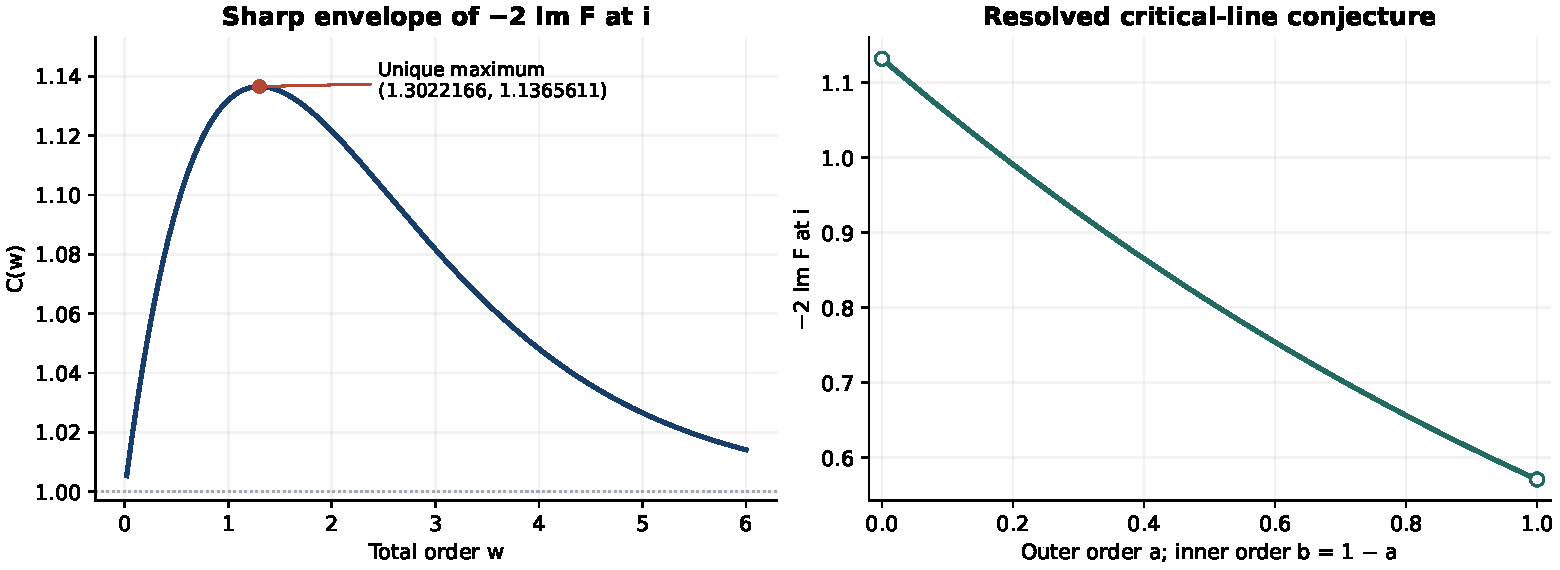
\includegraphics[width=\textwidth]{figures/gaussian_envelope.pdf}
\caption{The sharp Gaussian envelope and its critical-line allocation.
The curves are diagnostic plots; the shapes and the maximum enclosure
are established by Theorems~\ref{thm:allocation}--\ref{thm:globalenvelope}.
Open endpoint markers denote limiting values, not allowed parameter pairs.}
\label{fig:gaussian}
\end{figure}
% BEGIN included source: article/euler_secant.tex
\section{A positive secant kernel for every Euler remainder}
\label{sec:secant}
Let $a,b>0$, $w=a+b>0$, and let $R_N=2^N(E_N-g_{a,b})$
use the Euler partial sums defined in \eqref{eq:eulerdef}, now for arbitrary $a,b>0$. Define
\[
 H_N(s)=\frac{(1-s^{-2})^N}{1+s^{-2}},\qquad s\ge1.
\]
\begin{theorem}[Positive secant identity]
For every $a,b>0$, the Euler series converges absolutely to the analytic
value $g_{a,b}$. Its partial sums decrease strictly to that value.
For every integer $N\ge1$, with $V\sim\mathrm{Beta}(a,b)$,
\begin{equation}\label{secant:eq:remainder}
 R_N=\mathbb E\!\left[\frac1{\Gamma(w)}\int_0^\infty
 r^{w-1}\frac{H_N(e^r)-H_N(e^{Vr})}{e^r-e^{Vr}}\,dr\right].
\end{equation}
The quotient is positive for $0<V<1$. Its extension to $V=1$ is
$H_N'(e^r)$. Formula~\eqref{secant:eq:remainder} gives a positive
integral. When a finite signed Hausdorff representation exists, its
formula for the same remainder instead uses cancellation between
positive and negative parts. The positive secant formula also works
below the signed-measure threshold.
\end{theorem}
\begin{proof}

Start with the positive Mellin representation, where $f(n)=f_n$,
\[
 f(n)=\frac1{\Gamma(a)\Gamma(b)}\int_0^\infty\!\int_0^\infty
 u^{a-1}t^{b-1}\frac{e^{-u}}{e^t-1}
 \bigl(e^{-2nu}-e^{-2n(u+t)}\bigr)\,du\,dt.
\]
This is the finite geometric-sum formula for $H_{2n}^{(b)}$ followed
by the gamma integral for $(2n+1)^{-a}$. Applying the finite binomial
transform gives
\[
 -d_k=\frac1{\Gamma(a)\Gamma(b)}\int_0^\infty\!\int_0^\infty
 u^{a-1}t^{b-1}\frac{e^{-u}}{e^t-1}
 \left((1-e^{-2(u+t)})^k-(1-e^{-2u})^k\right)du\,dt.
\]
Every displayed integrand is nonnegative. Tonelli's theorem therefore
permits summing $\sum_{k\ge N}2^{N-k-1}(-d_k)$ under the double
integral. Summing the two geometric tails produces
\[
 \frac{e^{-u}}{e^t-1}
 \left(H_N(e^{u+t})-H_N(e^u)\right)
 =\frac{H_N(e^{u+t})-H_N(e^u)}{e^{u+t}-e^u}.
\]
The beta change of variables $r=u+t$, $v=u/r$ gives the asserted
integral for this nonnegative series. To establish its finiteness and
identify the Euler sum without a restriction on $w$, first take $N=1$.
Direct simplification shows that its secant kernel is twice the
kernel in \eqref{eq:Jw}. Therefore
\[
 \sum_{k\ge1}\frac{-d_k}{2^{k+1}}
   =\mathbb E J_w(V)=-g_{a,b}<\infty.
\]
This proves absolute convergence to the analytic value for every
positive pair. Also $d_k<0$ for $k\ge1$, since its displayed positive
integrand is strictly positive. Hence the partial sums decrease
strictly. Every later geometric tail is finite and equals
$2^N(E_N-g_{a,b})$, proving the formula for all $N\ge1$.
No conditionally convergent rearrangement is needed.
\end{proof}

For $N=1$, $H_1(s)=(s^2-1)/(s^2+1)$ and
\[
 H_1''(s)=\frac{4(1-3s^2)}{(1+s^2)^3}<0\qquad(s\ge1).
\]
Consequently its secant slope decreases as the lower endpoint $e^{vr}$
increases. Direct simplification gives
\[
 \frac{H_1(e^r)-H_1(e^{vr})}{e^r-e^{vr}}
 =\frac{e^{-vr}+e^{-r}}{2\cosh(vr)\cosh r},
\]
which is exactly twice the kernel used in the allocation theorem.
For $N=2$, however, $H_2(1+h)=2h^2+O(h^3)$, so $H_2$ is convex near
one. The same pointwise concavity proof does not extend to every $N$.

There is a particularly small exact obstruction to monotonicity in Euler
order away from the critical line. At $(a,b)=(1,1)$,
\[
 g_{1,1}=\operatorname{Im}\frac12\log^2(1-i)
       =-\frac{\pi\log2}{8},\qquad f(1)=\frac{H_2}{3}=\frac12.
\]
Since $E_1=0$ and $E_2=-f(1)/4=-1/8$,
\[
 R_1=\frac{\pi\log2}{4},\qquad
 R_2=\frac{\pi\log2}{2}-\frac12,
 \qquad R_2-R_1=\frac{\pi\log2-2}{4}>0.
\]
The last inequality follows already from $\pi>3$ and
$\log2=2\operatorname{artanh}(1/3)>2/3$.
This does not challenge the critical-line monotonicity theorem, whose
endpoint atom supplies a different argument. It shows why the sharp
bound for $-2g$ and the first Euler remainder cannot be declared the
sharp bound for every Euler order without an additional argument.

% END included source: article/euler_secant.tex

% BEGIN included source: article/cyclic.tex
% Standalone section. Requires amsmath, amssymb, amsthm and standard theorem environments.
% Source reviewed: ProveIt commit a0a90ef31877f98be437191c48b46f02d5456867.
\section{Cyclic prime symmetries and integral torsion}
\label{cpc:sec:main}

The incoming integral-distribution reports \cite{integraljets} determine reflection torsion
and explicitly propose a subgroup of prime order as a next target.
We solve that problem for an action which is trivial on one primary
factor and has no nonzero fixed point on the complementary factor,
assuming the fixed factor has semisimple unit-group action modulo the
symmetry prime. The result includes arbitrary integral weights and all
one-variable integral jets. Its obstruction is a finite multiplicative
compatibility condition, rather than a condition on each weight in
isolation.

The finite resolution and double-complex method have classical
antecedents in Kubert, Anderson, and Ouyang
\cite{cpc:Kubert1979,cpc:Ouyang2001,cpc:Ouyang2002}.
In particular, Ouyang's universal norm distributions already provide a
much broader setting for weighted distribution relations and their
cohomology. The calculation below is an explicit continuation for the
specified finite grid and a diagonal cyclic subgroup. We claim no global
priority for its ordinary-weight specialization or for the resolution
method.

\subsection{The formal module and the hypotheses}

For a commutative ring $B$, let $X_q=(1/q)\mathbb Z/\mathbb Z$ and
choose weights $a_p\in B$, one for each prime $p\mid q$. Define
\begin{equation}\label{cpc:eq:distribution}
 D_q(B,\mathbf a)=
 \frac{B[X_q]}{
 \left\langle\displaystyle\sum_{py=x}e_y-a_pe_x:
                    p\mid q,\ x\in X_{q/p}\right\rangle}.
\end{equation}
Every root sum is taken in $X_q$. The symbol $e_0$ is retained.
The integral normal-form theorem from the incoming reports, recalled
below with its proof mechanism, gives a $B$-free module of rank
$\varphi(q)$ for every specialization.

Let $\ell$ be a prime and let $u\in(\mathbb Z/q\mathbb Z)^\times$
have order $\ell$. Multiplication by $u$ induces
$T(e_x)=e_{ux}$. We impose the following explicit hypotheses:
\begin{equation}\label{cpc:eq:hypotheses}
 q=md,\qquad (m,d)=1,\qquad d>1,\qquad
 u\equiv1\pmod m,\qquad (u-1,d)=1,\qquad
 \ell\nmid\varphi(m).
\end{equation}
Here $\varphi(1)=1$. Necessarily $m=(u-1,q)$, so the factorization,
when it exists, is determined by $u$. The $T$-fixed grid is precisely
$X_m$. Write
\begin{equation}\label{cpc:eq:parameters}
 r=\omega(d),\qquad
 H=\langle p\bmod m:p\mid d\rangle
       \ \le (\mathbb Z/m\mathbb Z)^\times.
\end{equation}
The group modulo one is the trivial group.

For integer weights, call the constants \emph{compatible} when
\begin{equation}\label{cpc:eq:compatibility}
 p\bmod m\longmapsto \overline a_p\in\mathbb F_\ell^\times
 \quad(p\mid d)
\end{equation}
extends to a homomorphism $H\to\mathbb F_\ell^\times$.
In particular, all these residues must be nonzero. Equivalently,
every relation $\prod_{p\mid d}p^{n_p}\equiv1\pmod m$, with
$n_p\in\mathbb Z$, must satisfy
$\prod_{p\mid d}\overline a_p^{\,n_p}=1$.
Set
\begin{equation}\label{cpc:eq:multiplicity}
 c(\mathbf a)=
 \begin{cases}
 \varphi(m)/|H|,&\text{if \eqref{cpc:eq:compatibility} holds},\\
 0,&\text{otherwise}.
 \end{cases}
\end{equation}

\begin{theorem}[Integral cyclic-prime coinvariants]
\label{cpc:thm:scalar}
Assume \eqref{cpc:eq:hypotheses} and let all weights be integers.
Then
\begin{equation}\label{cpc:eq:scalar}
 \boxed{\displaystyle
 D_q(\mathbb Z,\mathbf a)/(T-1)D_q(\mathbb Z,\mathbf a)
 \simeq \mathbb Z^{\varphi(q)/\ell}
       \oplus (\mathbb Z/\ell\mathbb Z)^{\,c(\mathbf a)2^{r-1}}.}
\end{equation}
Consequently every nonunit nonzero Smith invariant of the complete
distribution-plus-symmetry presentation equals $\ell$, with the
multiplicity in \eqref{cpc:eq:scalar}. The answer is independent of
all weights $a_p$ with $p\mid m$.
\end{theorem}

\begin{corollary}[No nonzero fixed grid point]
\label{cpc:cor:fixedfree}
If $u$ has prime order $\ell$ and $(u-1,q)=1$, then
\[
 D_q/(T-1)D_q\simeq
 \mathbb Z^{\varphi(q)/\ell}\oplus
 \begin{cases}
 (\mathbb Z/\ell\mathbb Z)^{2^{\omega(q)-1}},
       &a_p\equiv1\pmod\ell\ \text{for every }p\mid q,\\
 0,&\text{otherwise}.
 \end{cases}
\]
For $\ell=2$ and odd $q$, this recovers the unanchored reflection
coinvariant formula. For $\ell>2$ it gives odd torsion.
\end{corollary}

The theorem describes a formal quotient. The equation $T=1$ is an
additional symmetry relation. Ordinary Hurwitz-zeta or polylogarithm
evaluation is not asserted to satisfy it without an appropriate
invariant projection. In particular, the finite torsion here is not
torsion of a complex-valued period and proves no numerical independence
statement.

\subsection{The finite resolution and its fixed part}

We record the algebra needed for a proof, including the role of the
prime-order assumption. Order the primes dividing $q$, and for a
subset $S$ put $p_S=\prod_{p\in S}p$. The weighted distribution
resolution has terms
\begin{equation}\label{cpc:eq:resolution}
 C_j=\bigoplus_{|S|=j}B[X_{q/p_S}],
 \qquad
 \partial[S,x]=\sum_{p\in S}(-1)^{\#\{v\in S:v<p\}}
 \left(\sum_{py=x}[S\setminus\{p\},y]
            -a_p[S\setminus\{p\},x]\right).
\end{equation}
Its augmentation is the quotient in \eqref{cpc:eq:distribution}.
The transfers and inclusions in different prime directions commute,
which gives $\partial^2=0$.

\begin{lemma}[Exactness over every coefficient ring]
\label{cpc:lem:resolution}
The augmentation of \eqref{cpc:eq:resolution} is exact. Its degree-zero
homology is $B$-free of rank $\varphi(q)$, and the augmented complex
is split exact as a complex of $B$-modules.
\end{lemma}
\begin{proof}
Here is the finite filtration argument, to make clear that no division
by $\ell$ or a prime weight is used. Filter $[S,x]$ by the positive
integer $p_S\operatorname{den}(x)$, which divides $q$. The leading
part of a prime differential retains only the preimages whose
denominator is multiplied by that prime; its weight term lies lower
in the filtration. At a fixed augmented denominator, additive primary
coordinates identify the leading complex with a tensor product of
maps
\[
 B[U_{p^{a-1}}]\longrightarrow B[U_{p^a}],
 \qquad e_b\longmapsto\sum_{v\mapsto b}e_v.
\]
At $a=1$, $U_1$ is a singleton and the sum has $p-1$ terms.
At $a>1$, each fiber has $p$ terms. In making this identification,
replace the $v$-primary coordinate in the $S$-summand by
$(\prod_{p\in S,\,p\ne v}p)^{-1}$ times that coordinate; this
removes the unit twists in the other primary components of a root.

Each displayed map is a split injection: its fibers have disjoint
support, and one coefficient-one pivot can be selected in each fiber.
Its cokernel is free of rank
$\varphi(p^a)-\varphi(p^{a-1})$. The tensor product is therefore
acyclic in positive degrees and has free degree-zero homology.
Lifting a leading boundary and subtracting it lowers the finite
filtration. This proves positive-degree exactness. The same lifting
in degree one proves that the image into degree zero is strict for
the filtration, so the chosen free complements lift to a basis of
the quotient. Their total number is
\[
 \prod_{p^e\parallel q}
 \left(1+\sum_{a=1}^{e}
      (\varphi(p^a)-\varphi(p^{a-1}))\right)=\varphi(q).
\]
Finally a surjection onto the free quotient splits; its kernel is
projective. Inducting upward splits the entire augmented complex.
\end{proof}

Let $C_j^{\rm mov}$ be generated by points which are not fixed by
$T$. It is a subcomplex: if $y$ is fixed, then $py$ is fixed, so a
root of a nonfixed point cannot be fixed. Since $T$ has prime order,
every nonfixed orbit has exactly $\ell$ elements, and each term of
$C_\bullet^{\rm mov}$ is a sum of regular cyclic permutation modules.
Put $K_\bullet=C_\bullet/C_\bullet^{\rm mov}$.

The fixed symbols in the summand indexed by $S$ form the grid
\[
 X_{m/p_{S\cap P(m)}}.
\]
For $p\mid m$, its fixed differential is the usual weighted
distribution differential. For $p\mid d$, exactly one root remains
fixed, namely $p^{-1}x$ in that grid. Thus this differential is
\begin{equation}\label{cpc:eq:fixedoperator}
 V_p-a_p,\qquad V_p(e_x)=e_{p^{-1}x}.
\end{equation}
All these operators commute. Applying Lemma~\ref{cpc:lem:resolution}
in the prime directions dividing $m$ shows that $K_\bullet$ is
quasi-isomorphic to the operator Koszul complex
\begin{equation}\label{cpc:eq:operatorKoszul}
 K\bigl(V_p-a_p:p\mid d;,D_m(B,\mathbf a|_m)\bigr).
\end{equation}
The notation means the tensor construction with one exterior
generator for each $p\mid d$, differential given by the indicated
commuting endomorphisms. The comparison follows by taking homology
first in the bounded $m$-directions; only degree zero survives.

\subsection{A cohomology formula which controls all torsion}

For a free abelian group $M$ with $T^\ell=1$, write
$\mathcal N=1+T+\cdots+T^{\ell-1}$ and define
\[
 \widehat H^0(M)=\ker(T-1)/\mathcal N M,
 \qquad
 \widehat H^1(M)=\ker\mathcal N/(T-1)M,
\]
extended periodically with period two. These are the cohomology
groups of the complex with differential $T-1$ leaving even degree
and $\mathcal N$ leaving odd degree.

\begin{lemma}[Torsion and the fixed complex]
\label{cpc:lem:tate}
For $B$ finite free over $\mathbb Z$ and $D=D_q(B,\mathbf a)$,
\begin{equation}\label{cpc:eq:torsiontate}
 \operatorname{Tor}_{\mathbb Z}(D/(T-1)D)
       =\widehat H^1(D).
\end{equation}
This group is killed by $\ell$. Under
\eqref{cpc:eq:hypotheses}, for $\epsilon\in\{0,1\}$ one has
\begin{equation}\label{cpc:eq:tateKoszul}
 \widehat H^\epsilon(D)\simeq
 \bigoplus_{j\equiv\epsilon\ ({\rm mod}\ 2)}
 H_j\!\left(
 K(V_p-\overline a_p:p\mid d;,
        D_m(B/\ell B,\overline{\mathbf a}|_m))\right).
\end{equation}
The isomorphism is one of $B$-modules; the right side is annihilated
by $\ell$.
\end{lemma}
\begin{proof}
If $kv=(T-1)w$ for a nonzero integer $k$, apply $\mathcal N$.
Freeness over $\mathbb Z$ gives $\mathcal N v=0$. Conversely,
if $\mathcal N v=0$, then $\ell v$ belongs to $(T-1)M$ because
$\ell-\mathcal N$ is divisible by $T-1$ in
$\mathbb Z[T]/(T^\ell-1)$. This proves both
\eqref{cpc:eq:torsiontate} and the annihilation assertion.

Apply the periodic cohomology complex to the finite resolution
\eqref{cpc:eq:resolution}. Taking horizontal homology replaces it
by $D$ in degree zero. A regular orbit has an exact periodic complex:
the image of $T-1$ is the coefficient-sum-zero subgroup, and the image
of $\mathcal N$ is the constant-vector subgroup. Hence removing
$C_\bullet^{\rm mov}$ does not change total cohomology. Both
comparisons are justified by finite horizontal width; each total
degree contains only finitely many summands.

On $K_\bullet$ the action is trivial, so the vertical complex
alternates between zero and multiplication by $\ell$. Since each
term of $K_\bullet$ is $\mathbb Z$-free, each adjacent
multiplication-by-$\ell$ block can be replaced by reduction modulo
$\ell$. The horizontal degree $j$ shifts total degree by $-j$,
which gives the parity in \eqref{cpc:eq:tateKoszul}. Finally use
the quasi-isomorphism \eqref{cpc:eq:operatorKoszul}, also after
reduction modulo $\ell$.
\end{proof}

\subsection{Proof of the scalar formula}

Let $k$ be an algebraic closure of $\mathbb F_\ell$. Since
$\ell\nmid\varphi(m)$, the character projectors for $U(m)$ are
defined over $k$. The conductor normal-form argument applies
verbatim in this characteristic: it only divides by unit-group
orders, and its edges do not divide by a weight or an Euler factor.
For clarity, the character $\chi$ has vectors
\[
 Y_{b,\chi}=\sum_{a\in U(b)}\chi(a)e_{a/b},
 \qquad \operatorname{cond}(\chi)\mid b\mid m.
\]
The prime edges are
$Y_{pb,\chi}-a_pY_{b,\chi}$ when $p\mid b$, and
$Y_{pb,\chi}-(a_p-\chi(p))Y_{b,\chi}$ when $p\nmid b$.
Successive elimination leaves exactly one conductor generator per
character. Therefore $D_m(k,\overline{\mathbf a})$ has one
one-dimensional summand for every character of $U(m)$, independently
of its weights. On that summand, $V_p$ acts by $\chi(p)$.

The complex in \eqref{cpc:eq:tateKoszul} consequently splits into
scalar Koszul complexes on
\begin{equation}\label{cpc:eq:characterparameters}
 (\chi(p)-\overline a_p:p\mid d).
\end{equation}
A nonzero scalar makes a Koszul complex contractible. If all these
scalars vanish, its differential is zero and its degree-$j$
homology has dimension $\binom rj$. Thus each surviving character
contributes $2^{r-1}$ to either cohomology parity.

The prescribed values in \eqref{cpc:eq:characterparameters} occur
if and only if \eqref{cpc:eq:compatibility} holds. A character of
the subgroup $H$ extends to $U(m)$ over $k$: one may successively
adjoin group elements and take the required roots in the algebraically
closed field. All relevant orders are prime to $\ell$. The set of
extensions is a torsor under the character group of $U(m)/H$, so
its cardinality is $\varphi(m)/|H|$. This proves the torsion
multiplicity in \eqref{cpc:eq:scalar}; extension to $k$ preserves
the dimension over $\mathbb F_\ell$.

For the free rank, rational coinvariants are an exact functor because
averaging over a finite group is possible over $\mathbb Q$. A
permutation set with $b$ points and $f$ fixed points has
$(b+(\ell-1)f)/\ell$ orbits. Its alternating count in the resolution
gives
\[
 \operatorname{rank}_{\mathbb Z}D/(T-1)D
 =\frac1\ell\sum_{S\subseteq P(q)}(-1)^{|S|}
 \left(\frac q{p_S}+(\ell-1)
           \frac m{p_{S\cap P(m)}}\right)
 =\frac{\varphi(q)}\ell.
\]
The second alternating sum vanishes because $r=\omega(d)>0$.
The classification of finitely generated abelian groups and
Lemma~\ref{cpc:lem:tate} complete the proof of
Theorem~\ref{cpc:thm:scalar}.

\subsection{All finite integral jets}

Let $B_L=\mathbb Z[t]/(t^L)$ with $L\ge1$, and take arbitrary
$a_p(t)\in B_L$. Test compatibility using the constant terms
$\overline a_p(0)$. If compatibility fails, put $c=0$ and
$\nu=0$. If it holds, let $c=\varphi(m)/|H|$ and define
\begin{equation}\label{cpc:eq:contact}
 \nu=\min_{p\mid d}
 \operatorname{ord}_t\bigl(\overline a_p(t)-\overline a_p(0)\bigr)
 \quad\text{in }\mathbb F_\ell[t]/(t^L),
 \qquad\operatorname{ord}_t(0)=L.
\end{equation}
In the compatible case $1\le\nu\le L$.

\begin{theorem}[Cyclic-prime integral jet formula]
\label{cpc:thm:jets}
Under \eqref{cpc:eq:hypotheses}, the underlying abelian group is
\begin{equation}\label{cpc:eq:jets}
 \boxed{\displaystyle
 D_q(B_L,\mathbf a)/(T-1)D_q(B_L,\mathbf a)
 \simeq\mathbb Z^{L\varphi(q)/\ell}
       \oplus(\mathbb Z/\ell\mathbb Z)^{\,c2^{r-1}\nu}.}
\end{equation}
More precisely, its integer torsion, as a $B_L$-module, is
\begin{equation}\label{cpc:eq:jetmodule}
 \left(B_L/(\ell,t^\nu)\right)^{c2^{r-1}}.
\end{equation}
The free summand in \eqref{cpc:eq:jets} is only asserted to be
free over $\mathbb Z$, not over $B_L$.
\end{theorem}
\begin{proof}
Over $k[t]/(t^L)$, the same conductor projectors split the fixed
module into free rank-one character blocks. A block whose constants
do not match has a unit parameter and is contractible. For each of
the $c$ matching characters, all parameters are the same list
\[
 -(\overline a_p(t)-\overline a_p(0)),\qquad p\mid d.
\]
In the principal ideal ring $k[t]/(t^L)$, invertible operations on
this list transform it into $(t^\nu,0,\ldots,0)$, interpreting
$t^L$ as zero. Both the kernel and the cokernel of multiplication
by $t^\nu$ are isomorphic to $k[t]/(t^\nu)$. Tensoring with the
$r-1$ remaining zero-differential exterior factors gives
\[
 H_j\simeq
 \left(k[t]/(t^\nu)\right)^{\binom rj}
\]
in each matching block. Lemma~\ref{cpc:lem:tate} gives the claimed
multiplicity.

For the $B_L$-module assertion no splitting-field ambiguity is
needed. The compatible character of $H$ takes values in
$\mathbb F_\ell$, so its averaging idempotent is defined over
$\mathbb F_\ell[t]/(t^L)$. Its image in the fixed distribution
module is a projective module of rank $c$ over this local ring,
hence is free of rank $c$. On that image every $V_p$ is the
prescribed scalar. The other character blocks are contractible
after the faithfully flat splitting extension and therefore have
zero homology already before that extension. The preceding scalar
Koszul calculation can consequently be performed over
$\mathbb F_\ell[t]/(t^L)$ itself, proving
\eqref{cpc:eq:jetmodule}. Finally the rational orbit count in the
scalar proof is multiplied by $L$, giving the free rank.
\end{proof}

\subsection{Explicit examples and boundaries of the result}

\paragraph{Level $91$, a genuinely odd torsion group.}
Take $q=7\cdot13$, $\ell=3$, and $u=16$. Then $u$ has order three
and $(u-1,91)=1$. For $a_7=a_{13}=1$,
\[
 D_{91}/(T-1)D_{91}\simeq\mathbb Z^{24}\oplus(\mathbb Z/3)^2.
\]
If either of these weights is not one modulo three, the torsion
vanishes. At jet length $L=4$, choose
$a_7(t)=1+t^2$ and $a_{13}(t)=1+3t+t^3$. Their contact order is
$\nu=2$, so the quotient is
$\mathbb Z^{96}\oplus(\mathbb Z/3)^4$.

\paragraph{Level $455$, a compatibility condition involving two primes.}
Take $q=5\cdot7\cdot13$, again with $\ell=3$ and $u=16$.
Here $m=5$, $d=91$, and
$H=\langle2,3\rangle=U(5)$ has order four.
Because $3=2^{-1}$ in $U(5)$ and every nonzero element of
$\mathbb F_3$ is its own inverse, compatibility is precisely
\[
 a_7\equiv a_{13}\not\equiv0\pmod3.
\]
Thus the quotient is
$\mathbb Z^{96}\oplus(\mathbb Z/3)^2$ when the two residues
are both one or both two, and is $\mathbb Z^{96}$ otherwise.
The value of $a_5$ is irrelevant. The case where both residues are
two shows why the criterion cannot be replaced by an independent
requirement $a_p\equiv1$ when a nontrivial fixed denominator remains.

\paragraph{The hypotheses exclude ramified local actions.}
At $q=9$, $\ell=3$, $u=4$, the fixed denominator is three, but it
is not relatively prime to its complementary factor. The five grid
orbits give generators $e_0,e_{1/3},e_{2/3},A,B$, where $A$ and
$B$ correspond to the two orbits of size three. The three raw
relations are
\[
 (1-a)e_0+e_{1/3}+e_{2/3}=0,\qquad
 3A-ae_{1/3}=0,\qquad 3B-ae_{2/3}=0.
\]
At $a=0,1,2$ these give, respectively,
\[
 \mathbb Z^2\oplus(\mathbb Z/3)^2,\qquad
 \mathbb Z^2\oplus\mathbb Z/3,\qquad
 \mathbb Z^2.
\]
These exact presentations explain why the fixed-grid hypotheses
must remain part of the statement. They are not counterexamples
to a claim in the inspected manuscript, which did not assert the
cyclic-prime formula.

\subsection{Verification, integration, and remaining questions}

The accompanying program constructs the complete defining rows
directly on $X_q$, identifies points in the orbits of $u$, and
computes the Smith normal form over $\mathbb Z$. It imports no
normal-form code from either incoming integral-distribution package.
Its frozen suite checks scalar weights for symmetry primes
$2,3,5$, prime-power and composite levels through $455$, incompatible
weight assignments, and nonconstant integral jets through length
four. The checks verify every nonzero invariant, not merely ranks
modulo $\ell$. They provide independent arithmetic regression
evidence; the all-level proofs are the arguments above.

The preceding exact results resolve the proposed prime-order subgroup
problem under \eqref{cpc:eq:hypotheses}. They do not settle it for an
arbitrary unit of prime order. Three concrete next problems remain.
First, compute the fixed complex for a local action of order $\ell$
on an $\ell$-power denominator, beginning with the displayed level-nine
presentation. Second, remove $\ell\nmid\varphi(m)$: the operator
Koszul model still applies, but its modular unit-group action need
not split into character lines. Third, compute the full module over
a multivariate deformation ring, where the scalar Koszul parameters
generate a nonprincipal ideal and a single contact order no longer
determines its homology. The first two problems concern new
stabilizer or modular representation structure; the third concerns
the syzygies of an explicit ideal.

% END included source: article/cyclic.tex

% BEGIN included source: article/lerch.tex
% Research contribution relative to ProveIt commit
% a0a90ef31877f98be437191c48b46f02d5456867 and its inspected incoming reports.
% Standalone section; use standard amsmath, amssymb, amsthm, booktabs, hyperref, graphicx.

\section{Resolvent order and a complete shape criterion for index two}
\label{lershape:sec:main}

The first-order index-two turning point and the complete index-three
phase diagram have already been proved in the incoming boundary and
global-phase reports~\cite{lershape:Boundary,lershape:Globalphase}.
They must not be presented as new conjectures here.
The results below add a finite-parameter comparison valid at every index,
and a shape classification valid at every derivative order at index two.
They also distinguish the second and third derivative orders rigorously:
the second-order lower zero still has an interior minimum, whereas both
third-order zeros decrease throughout the deformation interval.

\subsection{The spectral family and inherited analytic facts}

For integers $n\geq0$, $k\geq1$, write
\begin{align}
 P_k(t)&=\prod_{j=1}^k(1+t/j)=\sum_{i=0}^k e_i(k)t^i,\notag\\
 B_{n,k}(x)&=n!\sum_{i=0}^{\min(n,k)}e_i(k)\frac{x^{n-i}}{(n-i)!},\notag\\
 f_{n,k}(a)&=k!a^{-k-1}B_{n,k}(-\log a),\label{lershape:eq:elementary}\\
 F_{n,k}^{\rho}(a)&=\sum_{m\geq0}\rho^m f_{n,k}(a+m),
 \qquad 0\leq\rho\leq1.\label{lershape:eq:spectral}
\end{align}
At $\rho=1$ this is $(-1)^{n+k}\gamma_n^{(k)}(a)$ in the
Laurent convention of the manuscript. At $\rho<1$ it is the same signed
parameter derivative of the convergent Lerch coefficient. The classical
all-order parameter-derivative identities are established in
Coffey's work~\cite{lershape:Coffey}. The defining
series converges absolutely even at $\rho=1$, since
$f_{n,k}(x)=O(x^{-k-1}(1+\log^n x))$ at infinity. Its $a$ derivatives
converge locally uniformly, and
\begin{equation}\label{lershape:eq:a-derivative}
 (F_{n,k}^{\rho})'=-F_{n,k+1}^{\rho}.
\end{equation}

The Appell--Laplace representation in the manuscript is
\begin{equation}\label{lershape:eq:laplace}
 F_{n,k}^{\rho}(a)=\int_0^\infty
 \frac{x^ke^{-ax}}{1-\rho e^{-x}}Q_n(\log x)\,dx,
 \qquad
 \frac{e^{xt}}{\Gamma(1+t)}=\sum_{n\geq0}Q_n(x)\frac{t^n}{n!}.
\end{equation}
The reciprocal-gamma product makes $Q_n$ strictly real-rooted, and
Laplace variation diminution bounds the positive zero count by $n$,
including multiplicities. We retain that established result as the
analytic zero-count input. We shall also use the elementary endpoint
signs: $F_{n,k}^{\rho}>0$ near $a=0$ and
$\operatorname{sgn}F_{n,k}^{\rho}=(-1)^n$ for all sufficiently large $a$.
All positive zeros lie in a common compact interval at fixed $n,k$ as
$\rho$ ranges over $[0,1]$. The latter fact follows because the first
spectral term diverges positively at zero while the other terms are
uniformly bounded there, and all spectral terms have their eventual
common sign past the last elementary zero.

\subsection{A finite-parameter resolvent comparison}

\begin{theorem}[Resolvent identity and the last positive zero]
\label{lershape:thm:resolvent}
Fix $n\geq0$ and $k\geq1$. For $0\leq\rho_1<\rho_2\leq1$ and $a>0$,
\begin{equation}\label{lershape:eq:resolvent}
 F_{n,k}^{\rho_2}(a)=F_{n,k}^{\rho_1}(a)
 +(\rho_2-\rho_1)\sum_{j\geq1}\rho_2^{j-1}
 F_{n,k}^{\rho_1}(a+j).
\end{equation}
The series is absolutely convergent, including when $\rho_2=1$.
If $R_1$ is the largest positive zero at $\rho_1$, then
$F_{n,k}^{\rho_2}$ has no zero in $[R_1,\infty)$. Thus, whenever both
largest positive zeros exist,
\begin{equation}\label{lershape:eq:last-order}
 R(\rho_2)<R(\rho_1).
\end{equation}
Neither saturation nor simplicity is required. If the function has no
positive zero at $\rho_1$, it has none at any larger parameter either.

On every interval where the largest zero is simple it is differentiable
and satisfies $R'(\rho)<0$ for $0<\rho<1$.
\end{theorem}

\begin{proof}
Since $\rho_1<1$, the double series on the right of
\eqref{lershape:eq:resolvent} is absolutely convergent even at
$\rho_2=1$: the coefficient of $|f_{n,k}(a+r)|$, after absolute values
and collection by $r=j+m$, is at most $(1-\rho_1)^{-1}$.
The coefficient identity
\[
 (\rho_2-\rho_1)\sum_{j=1}^r\rho_2^{j-1}\rho_1^{r-j}
 =\rho_2^r-\rho_1^r
\]
then proves the resolvent formula term by term.

Put $\sigma=(-1)^n$. On $(R_1,\infty)$ the first function has
strict sign $\sigma$, because there are no more zeros. At every
$a\geq R_1$ all shifted values in the sum therefore have that same
strict sign. The unshifted value is either of sign $\sigma$ or zero.
Consequently $\sigma F_{n,k}^{\rho_2}(a)>0$ throughout this closed
ray. If no zero exists at $\rho_1$, the function has a fixed strict
sign on the whole positive axis and the same argument applies everywhere.

Differentiating the resolvent, or directly collecting the absolutely
convergent interior series, gives
\begin{equation}\label{lershape:eq:parameter-resolvent}
 \partial_\rho F_{n,k}^{\rho}(a)
 =\sum_{j\geq1}\rho^{j-1}F_{n,k}^{\rho}(a+j),\qquad 0\leq\rho<1.
\end{equation}
At a largest simple zero both $\partial_a F$ and every shifted value
have sign $\sigma$. Implicit differentiation yields
$R'=-F_\rho/F_a<0$.
\end{proof}

\begin{remark}[Scope of the finite comparison]
The largest zero can disappear in a multiple-zero event. The theorem
does not assert its continuity through such an event, nor does it
classify all possible inner folds. Its finite inequality applies
whenever the two largest zeros being compared exist. In particular it
gives strict decrease on $[0,1]$ for every largest-root family already
known to remain simple there.
\end{remark}

For later use, all interior parameter derivatives have a similar exact
formula. For $r\geq1$,
\begin{equation}\label{lershape:eq:higher-parameter}
 \partial_\rho^rF_{n,k}^{\rho}(a)
 =r!\sum_{j\geq r}\binom{j-1}{r-1}\rho^{j-r}
 F_{n,k}^{\rho}(a+j),\qquad 0\leq\rho<1.
\end{equation}
This follows either from \eqref{lershape:eq:laplace} and the geometric
series or by collecting coefficients. At a largest zero its sign is
$(-1)^n$ for every $r\geq1$. These are partial derivatives of $F$;
the statement does not say that every derivative of the zero location
has a fixed sign.

\subsection{Two coefficient sign changes allow only one turning point}

Put
\begin{equation}\label{lershape:eq:two-roots}
 H_k=\sum_{j=1}^k\frac1j,\qquad
 s_k=\left(\sum_{j=1}^k\frac1{j^2}\right)^{1/2},\qquad
 A_k=e^{H_k-s_k},\quad B_k=e^{H_k+s_k}.
\end{equation}
At index two the elementary kernel is
\begin{equation}\label{lershape:eq:f2}
 f_{2,k}(a)=k!a^{-k-1}\bigl((H_k-\log a)^2-s_k^2\bigr).
\end{equation}
Its sign pattern on the positive axis is $+,-,+$, with zeros $A_k,B_k$.
For a fixed $a$, the nonzero coefficients $f_{2,k}(a+m)$ therefore
have at most two sign changes as $m$ increases.

We recall the elementary power-series Descartes principle. A nonzero
real power series with $s$ coefficient sign changes has at most $s$
zeros in $(0,1)$ counted with multiplicity. For completeness, choose a
real cutoff $c$ between the coefficient indices at the first sign
change. The coefficients of $(\rho\partial_\rho-c)h$ have one fewer
sign change, since the first sign block is reversed. Its transform is
$\rho^{c+1}(\rho^{-c}h)'$. Induction and Rolle's theorem with
multiplicity prove the assertion, starting with a sign-definite series.
All differentiations are justified on compact subintervals of $(0,1)$.
In particular, a series whose nonzero coefficients are negative and
then positive has positive derivative at every interior zero: at a
separating cutoff $c$, every nonzero term of
$\sum_m(m-c)c_m\rho^m$ is positive.

The incoming index-two theorem gives exactly two simple positive zeros
of $F_{2,k}^{\rho}$ for every $k\geq1$ and $0\leq\rho\leq1$. We denote
them by $a_k(\rho)<b_k(\rho)$. A short reconstruction is useful. At
$k=1$ the exact rational evaluation in the present package gives
\[
 -0.07105864218565829478
 <F_{2,1}^{1}(13/10)
 <-0.07105864218565829477.
\]
At $a=13/10$ the spectral coefficients are negative and then positive.
The single-crossing coefficient argument keeps their sum negative for
all smaller parameters, including the elementary endpoint. Positive
signs near zero and infinity give two roots, and the global bound makes
both simple. Rolle's theorem between the roots, plus a stationary point
after the last one because $F$ tends to zero at infinity, preserves two
distinct roots at every higher derivative order. The same bound makes
them complete and simple.

\begin{theorem}[All-order shape dichotomy at index two]
\label{lershape:thm:dichotomy}
For each integer $k\geq1$ the upper branch $b_k$ is strictly decreasing
on $[0,1]$. The lower branch $a_k$ has at most one stationary point in
$(0,1)$. Any such point $\rho_*$ is a nondegenerate minimum:
\[
 a_k'(\rho_*)=0,\qquad a_k''(\rho_*)>0.
\]
It follows that exactly one of the following occurs:
\begin{enumerate}
\item $a_k'(\rho)<0$ for all $0<\rho<1$;
\item there is one $\rho_*\in(0,1)$, with $a_k'<0$ before it and
      $a_k'>0$ after it.
\end{enumerate}
In both cases the branch initially decreases. More explicitly, if
$d_k=\log(1+A_k^{-1})$, then
\begin{equation}\label{lershape:eq:initial-velocity}
 a_k'(0)=-\frac{A_k^{k+2}}{2s_k(A_k+1)^{k+1}}
                 d_k(2s_k-d_k)<0.
\end{equation}
\end{theorem}

\begin{proof}
Simplicity and compactness give continuous branches on $[0,1]$, analytic
for $0\leq\rho<1$. The upper assertion follows immediately from
Theorem~\ref{lershape:thm:resolvent}.

Consider a stationary point of the lower branch and fix its location
$a=a_k(\rho_*)$. If $a\geq B_k$, every spectral coefficient is
nonnegative and some are positive, so no zero is possible. If
$A_k\leq a<B_k$, the coefficients are negative and then positive,
after ignoring zeros. Their derivative is strictly positive at a zero,
so $F_\rho=0$ is impossible there. Hence $a<A_k$.

Now $h(\rho)=F_{2,k}^{\rho}(a)$ has positive constant term and at
most two coefficient sign changes. At the stationary point,
$h(\rho_*)=h'(\rho_*)=0$. Descartes' bound forces exact multiplicity
two and excludes every other parameter zero. Since $h(0)>0$, the
double contact has $h''(\rho_*)>0$. The lower root has $F_a<0$.
Twice differentiating the implicit equation at the stationary point
therefore gives
\[
 a_k''(\rho_*)=-\frac{F_{\rho\rho}}{F_a}>0.
\]
Every stationary point is consequently a strict minimum, with derivative
negative immediately before it and positive immediately after it.
There can be at most one: two would force a transition from positive
derivative to negative derivative at an intervening zero of the
derivative, contradicting the just-proved local behavior.

At $\rho=0$, implicit differentiation yields
$a_k'(0)=-f_{2,k}(A_k+1)/f_{2,k}'(A_k)$. Here
$f_{2,k}'(A_k)=-2s_k k!A_k^{-k-2}$, which gives
\eqref{lershape:eq:initial-velocity}. Its strict sign follows from
$A_k+1<B_k$: indeed
$B_k-A_k=2e^{H_k}\sinh s_k\geq2e\sinh1>1$.
This also gives $0<d_k<2s_k$ and completes the dichotomy.
\end{proof}

\subsection{The entire shape is determined by one endpoint sign}

For $k\geq2$, the series for $F$ and $F_\rho$ converge absolutely and
locally uniformly in $a$ at $\rho=1$. Thus both zero branches are $C^1$
on $[0,1]$. Put $r_k=a_k(1)$ and define
\begin{equation}\label{lershape:eq:Ck}
 C_k(a)=kF_{2,k-1}^{1}(a)+2F_{1,k-1}^{1}(a).
\end{equation}

\begin{theorem}[Endpoint criterion]
\label{lershape:thm:criterion}
For every integer $k\geq2$,
\begin{equation}\label{lershape:eq:endpoint-velocity}
 a_k'(1)=\frac{C_k(r_k)}{F_{2,k+1}^{1}(r_k)}.
\end{equation}
The denominator is strictly positive. The lower branch has its unique
interior minimum if and only if $C_k(r_k)>0$. If $C_k(r_k)\leq0$,
then $a_k'(\rho)<0$ for every $0<\rho<1$.
\end{theorem}

\begin{proof}
The elementary generating identity
\[
 (a+m)\,f_{n,k}(a+m)
 =k f_{n,k-1}(a+m)+n f_{n-1,k-1}(a+m)
\]
follows by differentiating $(k+t)(1+t)_{k-1}(a+m)^{-k-t}$ in
$t$ exactly $n$ times at zero. Summing it gives, for $k\geq2$,
\begin{equation}\label{lershape:eq:rho-endpoint}
 \partial_\rho F_{n,k}^{1}(a)
 =kF_{n,k-1}^{1}(a)+nF_{n-1,k-1}^{1}(a)-aF_{n,k}^{1}(a).
\end{equation}
Use $n=2$, $F_{2,k}^{1}(r_k)=0$ and
$F_a=-F_{2,k+1}^{1}$ to obtain
\eqref{lershape:eq:endpoint-velocity}. The denominator is positive
because $F_a<0$ at the lower simple root.

If this velocity is positive, the negative initial velocity and
continuity force a stationary point; the dichotomy gives precisely one.
If it is negative, an interior minimum is impossible, since after the
only possible minimum the derivative would remain positive all the way
to the endpoint.

We include the zero-velocity case to make the criterion complete.
Suppose $a_k'(1)=0$. Set $r=r_k$ and $h(\rho)=F_{2,k}^{\rho}(r)$.
Then $h(1)=h'(1)=0$. If $r\geq A_k$, the single-crossing argument
would instead give $h'(1)>0$; the sums with the additional factor $m$
are absolutely convergent, so the same strict weighted-coefficient
proof applies at the endpoint. Hence $r<A_k$, and the nonzero
coefficients of $h$ have the pattern $+,-,+$.

Choose $c$ between the last negative coefficient index and the first
following positive index, and put $p=(\rho\partial_\rho-c)h$.
Its nonzero coefficients have the single pattern $-,+$ and
$p(1)=0$. The weighted single-crossing inequality implies
$p(\rho)<0$ for all $0<\rho<1$: an appropriate power of $\rho$
times $p$ is strictly increasing to zero at one. Therefore
\[
 (\rho^{-c}h)'=\rho^{-c-1}p<0,
 \qquad \lim_{\rho\uparrow1}\rho^{-c}h(\rho)=0,
\]
and $h(\rho)>0$ on $(0,1)$. If the lower branch had an interior
minimum, it would increase thereafter toward $r$; sufficiently near
one, $a_k(\rho)<r<b_k(\rho)$ and hence $h(\rho)<0$, a contradiction.
The zero-velocity case also has no interior minimum. The dichotomy
then makes its derivative strictly negative at every interior point.
\end{proof}

The first derivative order can also be recovered directly from these
arguments. In \eqref{lershape:eq:laplace}, at $n=2,k=1$, the integrand
of $F_\rho$ is
\[
 \frac{x e^{-(a+1)x}}{(1-\rho e^{-x})^2}
 \bigl((\log x+\gamma)^2-\zeta(2)\bigr).
\]
Its negative part is supported in a fixed compact interval away from
zero and has bounded integral, uniformly for $a$ in a fixed compact
positive interval. Its positive part near zero increases to a function
asymptotic to $x^{-1}\log^2 x$, which has divergent integral. Hence
$F_\rho\to+\infty$ as $\rho\uparrow1$, uniformly along the compact
lower-root branch. Since $F_a$ stays negative and away from zero near
its simple endpoint, $a_1'(\rho)>0$ near one. Together with the initial
negative derivative and Theorem~\ref{lershape:thm:dichotomy}, this
reproves the incoming first-order minimum theorem without assuming a
numerical minimum scan.

\subsection{The second-order reversal and third-order decrease}

\begin{theorem}[A rigorously separated pair of derivative orders]
\label{lershape:thm:k2k3}
The second-order lower branch $a_2$ has exactly one nondegenerate
interior minimum. The third-order lower branch $a_3$ decreases strictly
throughout $[0,1]$, and $a_3'(\rho)<0$ at every interior parameter.
The upper branch decreases at both orders. Consequently $k=3$ is the
smallest individual derivative order for which both index-two branches
decrease throughout the interval; the incoming first-order theorem and
the present second-order theorem exclude $k=1,2$.

The following are rigorous rational enclosures:
\begin{align*}
 1.29982837988436&<r_2<1.29982837988437,\\
 1.77628448580819&<r_3<1.77628448580820,\\
 0.02581658837068013&<a_2'(1)<0.02581658837071208,\\
 -0.24231787997240310&<a_3'(1)<-0.24231787997233853.
\end{align*}
\end{theorem}

\begin{proof}
Exact arithmetic gives positive and negative endpoint signs,
respectively, at the ends of each displayed root interval. The
two-zero theorem makes each positive-to-negative crossing the lower
simple zero. On the entire root intervals, the same arithmetic encloses
\begin{align*}
 -2.158373629377&<F_{2,2,a}^{1}<-2.158373629376,\\
 0.0557218435397&<C_2<0.0557218435399,\\
 -1.066689311681&<F_{2,3,a}^{1}<-1.066689311680,\\
 -0.2584778925956&<C_3<-0.2584778925955.
\end{align*}
The full unrounded intervals give the displayed velocity enclosures.
The signs are therefore valid at the unknown exact roots, and
Theorem~\ref{lershape:thm:criterion} proves the asserted global shapes.
\end{proof}

A separate, non-interval Laplace-integral diagnostic locates the new
minimum at
\[
 \rho_*\approx0.9998163851082947468,
 \qquad a_2(\rho_*)\approx1.299826525290189674.
\]
The diagnostic gives $a_2''(\rho_*)\approx86.8818201681$. These
decimals are not claimed to be certified minimum enclosures. The
existence, uniqueness and nondegeneracy of the minimum follow from the
theorems and the exact endpoint signs, not from this numerical solve.
The narrow upturn also explains why a coarse parameter grid can miss
the second-order failure of monotonicity.

\begin{figure}[htbp]
\centering
\IfFileExists{../figures/lerch_shape_diagnostic.pdf}{%
  \includegraphics[width=\textwidth]{../figures/lerch_shape_diagnostic.pdf}}{%
  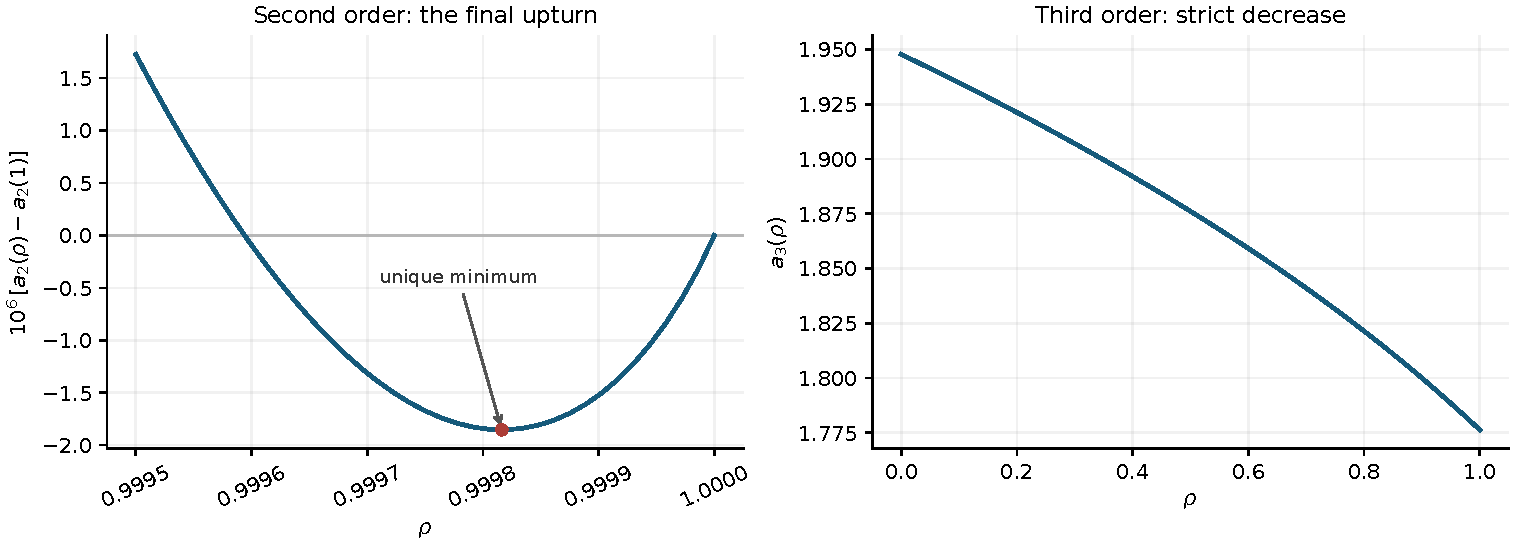
\includegraphics[width=\textwidth]{figures/lerch_shape_diagnostic.pdf}}
\caption{Numerical diagnostics of the proved shapes. Left: the final
second-order upturn, on a scale of one million times the difference
from the endpoint root. Right: the third-order lower branch. The red
minimum marker is the independent Laplace-integral diagnostic. All 79
plotted points and their spectral-tail majorants are retained in
\texttt{results/lerch/shape\_plot\_points.csv}; arithmetic rounding is
not enclosed. The existence and shape theorems rely on the analytic
proofs and exact endpoint certificates.}
\label{lershape:fig:shape}
\end{figure}

The last statement of Theorem~\ref{lershape:thm:k2k3} concerns the
smallest individual order. A proof that the same property holds for
\emph{every} $k\geq3$ remains a separate question. The inherited
eventual-monotonicity theorem proves it for all sufficiently large $k$;
the endpoint criterion reduces the sharp remaining assertion to
$C_k(r_k)\leq0$ for each $k\geq3$.

\subsection{Exact certificate and its analytic error bound}

The proof-bearing computation is
\texttt{code/lerch/certify\_shape.py}, using the exact-rational engine
\texttt{code/lerch/exact\_engine.py}. It uses $N=32$ initial summands,
$p=8$ Bernoulli corrections, $90$ logarithm-series terms and outward
rounding to the fixed grid $10^{-70}\mathbb Z$. The complete rational
data are in \texttt{results/lerch/shape\_certificates.json}. The engine is
copied from the incoming boundary report; the new code adds whole-interval
endpoint evaluation and the endpoint shape certificates.

Euler--Maclaurin evaluation of Hurwitz-zeta derivatives with rigorous
error bounds also has an established algorithmic literature, notably
Johansson~\cite{lershape:Johansson}. Here is the particular analytic
contract used for our rational certificate. If $b=a+N$, the
Euler--Maclaurin formula and $f_{n,k}'=-f_{n,k+1}$ give
\begin{align}\label{lershape:eq:EM}
 F_{n,k}^{1}(a)={}&\sum_{m=0}^{N-1}f_{n,k}(a+m)
 +f_{n,k-1}(b)+\frac12f_{n,k}(b)\notag\\
 &+\sum_{j=1}^{p}\frac{B_{2j}}{(2j)!}f_{n,k+2j-1}(b)+R.
\end{align}
Write $s=k+2p$ and
$B_{n,s}(x)=\sum_{q=0}^n c_qx^q$, where every $c_q\geq0$. The
periodic Bernoulli remainder and an elementary integral give
\begin{align}\label{lershape:eq:EM-bound}
 |R|&\leq\frac{|B_{2p}|s!}{(2p)!}
 \sum_{q=0}^nc_q\int_b^\infty x^{-s-1}\log^q x\,dx,\notag\\
 \int_b^\infty x^{-s-1}\log^q x\,dx
 &=b^{-s}\sum_{j=0}^q
 \frac{q!}{(q-j)!}\frac{\log^{q-j}b}{s^{j+1}}.
\end{align}
All instances use $b>1$. For an interval of possible $a$ values, natural
outward interval arithmetic is applied to every finite term of
\eqref{lershape:eq:EM}; evaluating the positive integral bound from
the smaller $b$ gives a valid bound for the whole interval. This is what
certifies $C_k$ at the actual root rather than only at a rounded root.

The logarithm is range-reduced to $1\leq y\leq2$, then evaluated by
\[
 \log y=2\sum_{j=0}^{M-1}\frac{u^{2j+1}}{2j+1}+R_M,
 \quad u=\frac{y-1}{y+1},\qquad
 0\leq R_M\leq\frac{2u^{2M+1}}{(2M+1)(1-u^2)}.
\]
Every number in the acceptance calculation is rational. The JSON file
records rational interval endpoints and their outward decimal displays;
no floating-point sign enters the theorem.

\subsection{Further questions and editorial consequences}

\begin{enumerate}
\item Prove or refute $C_k(r_k)<0$ for every $k\geq3$. This is a
      concrete all-order inequality in classical Stieltjes derivatives,
      exactly equivalent to the proposed sharp persistent monotonicity
      threshold once the possible equality case is included.
\item Derive a recurrence or comparison inequality in $k$ for
      $C_k(r_k)$. Such a comparison would turn the third-order certificate
      into an all-higher-order theorem, avoiding an unlimited list of
      finite checks.
\item Certify a narrow two-dimensional box for the second-order minimum.
      The parameter $\eta=-\log\rho$ and the existing Abel singularity
      subtraction are suitable coordinates; a raw geometric truncation
      converges slowly at the observed parameter.
\item Extend the resolvent comparison from the largest zero to selected
      inner zeros using additional sign information on the shifted
      values. The formula already specifies exactly which weighted
      tail controls a root's velocity.
\item Determine which discontinuities of the largest-root function can
      occur at higher indices. Strict finite-parameter order excludes
      an upward jump; classifying possible losses of the outermost pair
      requires information beyond the order theorem.
\end{enumerate}

No inspected proof of the existing first-order shape or the eventual
monotonicity theorem is contradicted. The editorial correction is to
keep three statements distinct: first-order nonmonotonicity, the new
second-order nonmonotonicity, and third-order strict decrease. A claim
that the eventual threshold is exactly three still needs the all-$k$
inequality in the first question. Likewise, the earlier formal-reductions
report's open first-order minimum question has already been settled by
the incoming boundary report and should be cross-referenced accordingly.

% END included source: article/lerch.tex

% BEGIN included source: article/s6_obstruction.tex
\section{A certified obstruction in the weight-seven reduction search}
\label{s6bounded:sec}

The weight-seven identity in the pinned manuscript \cite{repo} remains conjectural.
Here $S_6=\sum_{n\ge0}(-1)^nH_n/(2n+1)^6$ and $H_0=0$.
Its equivalent short form is
\begin{align}
 S_6={}&-\frac{12334}{527}g_{6,1}-\frac{384}{31}g_{5,2}
 -\frac{2136}{527}g_{4,3}+\frac{3179\pi^7}{5713920}\notag\\
 &-\frac{801}{2108}\beta(4)\zeta(3)-2\beta(6)\log2.
 \label{s6bounded:eq:conjecture}
\end{align}
The earlier formal obstruction involves products of two single values.
We tested a substantially larger finite family, allowing double-shuffle
rows through depth four, convergent distribution and its lifts,
products of the already proved $S_2$ and $S_4$ relations, and a specified
family of Cayley identities whose expansions stay within depth four.
An exact integer functional separates the target from this enlarged
span. This is a result about the stated formal presentation; it neither
disproves the numerical conjecture nor excludes identities outside that
presentation.

Use the forms
\[
 z=dt/t,\quad c=dt/(1-t),\quad
 A=i\,dt/(1-it),\quad B=-dt/(1+t),\quad
 \bar A=-i\,dt/(1+it),
\]
and outer-letter-first iterated integrals on $[0,1]$. Admissible words
have first letter different from $c$ and last letter different from $z$.
Their depth is the number of letters different from $z$. Let $\mathcal W$
be the rational space on imaginary admissible words of weight seven and
depth at most four, with conjugates identified with opposite signs.
It has dimension $2546$. More explicitly, the dimensions at exact
depths one through four are $1,35,390,2120$; they count formal words,
not independent periods.

The interval-reversing Cayley substitution $\phi(t)=(1-t)/(1+t)$
acts by reversal and the
letter map
\[
 \tau z=c-B,\quad \tau c=z+B,\quad
 \tau A=B-\bar A,\quad \tau B=B,\quad
 \tau\bar A=B-A.
\]
The displayed letter map is $\tau=-\phi^*$, with the reversed
orientation included; it is not the unadjusted pullback. Regularized
double shuffle is used with the standard single-divergence convention
\cite{zhao,racinet}.
It becomes especially convenient on the combinations
\begin{gather*}
 x=c-B,\qquad y=A-\bar A,\qquad h=A+\bar A-B,\\
 \tau z=x,\quad\tau x=z,\quad\tau y=y,\quad
 \tau h=-h,\quad\tau B=B.
\end{gather*}
For an abstract word $u$ on $\{z,x,y,h,B\}$ let $\widehat u$ denote
its expansion in the original alphabet. If its first letter is not
$x$ and its last letter is not $z$, every expanded word and every
Cayley-transformed expanded word is admissible. If $u$ has length $l$
and contains $n_z$ copies of $z$ and $n_x$ copies of $x$, the two
expansions have depths at most $l-n_z$ and $l-n_x$. In particular,
the $z^3x^3y$ permutations supply weight-seven Cayley rows that remain
in $\mathcal W$ on both sides. This is a useful way to add geometric
relations without immediately introducing all depth-seven coordinates.

The certificate fixes the following finite row family. Each row is
projected to its imaginary part, nonzero rational multiples are
identified, and duplicates are removed.
\begin{enumerate}
\item All weight-seven shuffle-minus-stuffle rows whose two input
      depths sum to at most four. Inputs are admissible, except that
      one factor may be $\operatorname{Li}_1(1)$, using the standard
      one-divergence comparison whose divergent word cancels.
\item All convergent level-two-to-level-four distribution rows,
      and their products with admissible words, when total weight is
      seven and the sum of depths is at most four. Products are
      expanded by stuffle. In relative-color notation, the seed is
      \[
      Z(\boldsymbol s;2\boldsymbol c)
      -2^{|\boldsymbol s|-d}
        \sum_{\boldsymbol\epsilon\in\{0,2\}^d}
        Z(\boldsymbol s;\boldsymbol c+\boldsymbol\epsilon),
      \qquad c_j\in\{0,1\}.
      \]
\item The imaginary $S_2$ and $S_4$ relations already proved in the
      manuscript, multiplied by real parts of all admissible words
      of the complementary weight, with total depth at most four.
\item For every $1\le l\le7$, every abstract word $u$ as above with
      $\min(n_z,n_x)\ge1$, take its convergent Cayley row and multiply
      it by each admissible word of weight $7-l$, provided
      $l-\min(n_z,n_x)$ plus the multiplier's depth is at most four.
      The empty multiplier is allowed when $l=7$.
\end{enumerate}
This prescription gives $5131$ distinct nonzero rows: $3460$ in the
first family, $1394$ newly added distribution rows, $40$ newly added
$S_2/S_4$ lifts, and $237$ newly added balanced Cayley lifts.
``Newly added'' here concerns duplicate removal in this finite row list,
not claims of new mathematical identities.

Let $T\in\mathcal W$ represent $128588$ times the left side minus the
right side of~\eqref{s6bounded:eq:conjecture}. The normalization uses
$S_6=g_{6,1}+\operatorname{Im}\operatorname{Li}_{6,1}(i,-1)$ and
$\beta(7)=61\pi^7/184320$. Before projecting and expanding the two
products, it is
\begin{align*}
 T=\operatorname{Im}\{&128588\operatorname{Li}_{6,1}(i,-1)
 +3138084\operatorname{Li}_{6,1}(i,1)
 +1592832\operatorname{Li}_{5,2}(i,1)\\
 &+521184\operatorname{Li}_{4,3}(i,1)
 -216172\operatorname{Li}_7(i)
 +48861\operatorname{Li}_4(i)\operatorname{Li}_3(1)\\
 &-257176\operatorname{Li}_6(i)\operatorname{Li}_1(-1)\}.
\end{align*}
Here $T$ denotes the corresponding formal vector, not its as-yet
unproved evaluation as a number.

\begin{theorem}[A finite enlarged-span obstruction]
The target $T$ does not belong to the rational span of the $5131$
rows specified above.
\end{theorem}
\begin{proof}
The supplementary file \texttt{S6\_depth\_bounded\_separator.json}
contains an integer functional $\ell$ on $\mathcal W$. The independent
program \texttt{verify\_s6\_separator.py} reconstructs every prescribed
row from its descriptor, using placement shuffles and stack-enumerated
index merges. It checks admissibility, weight seven, and depth at most
four. For Cayley rows it performs the raw five-letter substitution,
independently of the diagonalized-letter shortcut used during discovery.
It also independently re-enumerates the full prescribed family and verifies
that its normalized row set equals the stored descriptor list. It then
verifies, using only integers, that every row $R$ has
$\ell(R)=0$, whereas $\ell(T)\ne0$. The explicit nonzero pairing is
recorded in the receipt. Linear algebra now proves the assertion.
The replay uses no rank assumption, modular arithmetic, numerical
polylogarithm, or integer-relation search.
\end{proof}

This certificate narrows one proof-search strategy. The family is still
smaller than all relations obtainable through arbitrary higher-depth
elimination. Even within a depth-bounded ansatz, other convergent linear
combinations of Cayley words need not be generated by these balanced
seeds. Thus the theorem does not prove that every possible proof must
pass through depth five. Its concrete recommendation is to enlarge
this specified row family or change its coordinate system, rather than
repeat the same search at higher numerical precision.

% END included source: article/s6_obstruction.tex

% BEGIN included source: article/audit_agenda.tex
\section{Verification, editorial reconciliation, and integration}
\label{sec:audit}

\subsection{What the computations establish}

The analytic theorems are proved in the text. Exact computation enters
at three clearly identified places: enclosure of the Gaussian maximum,
endpoint signs for the two Lerch branch-shape decisions, and separation
of a finite formal relation span. The distribution examples and inverse
coefficient checks are independent consistency tests of general proofs.

\begin{longtable}{@{}L{0.24\textwidth}L{0.37\textwidth}L{0.32\textwidth}@{}}
\toprule
Check & Construction & Logical role\\
\midrule
\endhead
Gaussian maximum & Outward rational intervals, finite Euler transforms,
analytic derivative tails & Certifies the printed root and maximum
intervals once strict log-concavity is proved.\\[4pt]
Inverse expansion & Exact symbolic generalized series, with exponents
encoded by rational bases & Substitution cancels every coefficient below
exponent two; the all-order theorem has an analytic proof.\\[4pt]
Cyclic quotients & Exact Smith forms of the original orbit relation
matrices, without a normal-form implementation & 52 scalar and finite-jet
cases check the theorem; three ramified examples test its boundary.\\[4pt]
Lerch branch shapes & Exact Euler--Maclaurin intervals on entire rational
root brackets & Certifies the signs deciding the order-two and
order-three global branch shapes.\\[4pt]
$S_6$ separation & Integer functional, independent row reconstruction
and complete-family enumeration & Proves nonmembership in the stated
5,131-row rational span.\\[4pt]
Plots and quadrature & Floating-point evaluation of independent
integrals and asymptotic formulas & Diagnostic evidence only; no claimed
certificate follows from a plot or an unenclosed decimal.\\
\bottomrule
\end{longtable}

The nine Gaussian comparison points evaluate the original Euler
transform and an independent beta-mixture quadrature. Their largest
observed discrepancy is below $6\cdot10^{-12}$ with the supplied
quadrature settings. This is a diagnostic discrepancy, not a proved
bound on the quadrature error. Four inverse examples compare the exact
coefficient formula with numerical solutions. The Lerch plot retains
its sampled values and analytic omitted-function estimates; floating
rounding is explicitly unenclosed. In particular, the diagnostic
coordinates of the order-two minimum are not a certified isolating box.
Its existence, uniqueness, and nondegeneracy are theorems independently
of those coordinates.

The programs and receipts are included in the archive. Running
\path{code/replay_all.py} from the package root regenerates all exact
receipts. Optional plotting dependencies are separated from the exact
arithmetic dependencies. No network access or numerical
integer-relation search is needed for the replay. The distribution
checks use SymPy's exact integer Smith algorithm; the Gaussian, Lerch,
and $S_6$ certificate arithmetic uses the Python standard library.

This is stronger than reporting successful high-precision fitting,
but it remains ordinary mathematical proof with auditable programs.
Formal verification in a proof assistant is a separate project. For
that project, the integer separator is an especially small logical
target: the checker need only reconstruct finite vectors and evaluate
integer dot products.

\subsection{Concrete proposed status corrections}

The reviewed material did not reveal a new counterexample to an
already established upstream theorem in the portions used here.
The useful corrections concern cross-report status and the scope of
claims made while integrating results.

\paragraph{Promote the critical constant conjecture.}
In \cite{realorder}, replace the status of Conjecture
\texttt{conj:constant} by a theorem, with the proof through
Theorems~\ref{thm:allocation} and \ref{thm:criticalconstant}.
Retain the analytic/Abel convention on $a+b=1$ and the endpoint atom.
The constant is a supremum over the open parameter interval, approached
as $a\downarrow0$; there is no admissible maximizing pair on the line.

\paragraph{Reconcile the first-order Lerch minimum.}
The formal-reductions report \cite{formalreductions} still lists
uniqueness of the smaller $n=2,k=1$ branch minimum as Conjecture
\texttt{research:conj:minimum}. The incoming boundary report
\cite{lershape:Boundary} proves that uniqueness. A combined manuscript
should cite the latter result and remove the obsolete open status.
The present contribution is the all-$k$ dichotomy, the endpoint
criterion, the order-two minimum, and the order-three decreasing
case. These should not be described as the first proof of the
already settled $k=1$ case.

\paragraph{Keep the $S_4$ and $S_6$ statuses distinct.}
The current manuscript has a proof chapter for $S_4$ and an explicitly
conjectural $S_6$ reduction in
\path{chapters/04-cyclotomic-quotients.tex}. The exact separator in
Section~\ref{s6bounded:sec} is a theorem about one finite presentation.
It supplies neither a proof nor a disproof of the $S_6$ evaluation.
Its enlarged row family should replace a repeated search in the same
smaller ansatz, rather than change the conjecture's numerical status.

\paragraph{Separate two different Euler constants.}
The global constant $C_*$ controls $-2g_{a,b}$ over all positive orders.
The critical constant $\pi/4+(\log2)/2$ controls every normalized Euler
tail on $a+b=1$. The exact $(a,b)=(1,1)$ calculation in
Section~\ref{sec:secant} proves that normalized errors need not decrease
off the critical line. This is a warning against an additional claim,
not a counterexample to either theorem stated here or to an identified
upstream theorem.

\paragraph{State the cyclic hypotheses where the formula is used.}
The restrictions $(m,d)=1$, $(u-1,d)=1$, and
$\ell\nmid\varphi(m)$ are part of the theorem. They should accompany
any extracted formula or summary. The level-nine computation shows
why a partially fixed primary factor is a distinct local problem.
Likewise, the term ``rank'' should specify whether it is a free
abelian rank, a formal rational dimension, or a rank after reduction
modulo a prime. No one of these determines the others without a proof.

\subsection{Suggested repository placement}

The complete report can first be placed under
\path{Analysis/Polylogarithms/docs/reports/extremal-bounds-cyclic-descent/}.
The integration guide supplies a compact addendum and a dependency
map. The natural manuscript neighborhoods are:
\begin{itemize}
\item Gaussian allocation, the critical Euler theorem, and the secant
identity next to the signed-kernel material and the real-order report;
\item the cyclic theorem and finite jets next to
\path{08-distribution.tex} and \path{08-conductor-jets.tex};
\item the Lerch branch theorems next to
\path{09-zero-geometry.tex} and the incoming boundary analysis;
\item the finite $S_6$ obstruction next to
\path{04-cyclotomic-quotients.tex} and the established $S_4$ proof.
\end{itemize}
The manuscript need not absorb the entire report at once. Its theorem
statements and their proof dependencies can be integrated by topic,
while the exact checkers and complete provenance remain with the report.
No repository mutation is part of this deliverable.

\section{Further research questions and proposed directions}
\label{sec:research}

The questions below are intentionally differentiated. Some preserve
existing conjectures, some ask for stronger theorems suggested by the
present proofs, and some concern a concrete missing computation.
No conjecture in this section is used earlier.

\subsection{Sharp bounds for the entire Euler scheme}

\paragraph{1. Optimize every normalized remainder.}
For $N\ge1$, determine
\[
 M_N=\sup_{a,b>0,\ a+b\ge1}2^N(E_N-g_{a,b}),
 \qquad M=\sup_{N\ge1}M_N.
\]
We have determined $M_1=C_*$. On the critical line the corresponding
all-$N$ supremum is $\pi/4+(\log2)/2$. The positive secant identity
reduces the general problem to a beta average of divided differences
of $H_N$. The main obstacle is concrete: $H_1$ is concave on
$[1,\infty)$, whereas $H_2$ is convex near one. A useful next step is
to locate the inflection structure of $H_N$ exactly and determine
whether its Mellin integral restores monotonicity in the allocation
parameter. We make no untested assertion that $M=C_*$.

\paragraph{2. Quantify allocation monotonicity.}
The covariance formula proves a strict sign but does not give a sharp
modulus. Find useful two-sided estimates for
\[
 -\frac{d}{da}\{-g_{a,w-a}\}
 =-\operatorname{Cov}\!\left(J_w(V_a),
                          \log\frac{V_a}{1-V_a}\right),
\]
uniformly near $a=0$ or $a=w$, or as $w\to0$ and $w\to\infty$.
The endpoint beta laws concentrate at different rates and have
logarithmic score singularities. Deriving a full endpoint expansion
would turn the sharp inequalities into effective error estimates for
nearly extremal orders. It would also test whether higher derivative
signs hold on a restricted range; they do not follow from stochastic
ordering alone.

\paragraph{3. Extend the allocation principle to other arguments.}
For $z=e^{i\theta}$ the positive double integral still supplies an
explicit rational imaginary kernel, but its dependence on the
allocation variable can change sign and shape with $\theta$.
Characterize the angles for which an appropriate signed component is
monotone at fixed total order. This would connect the Gaussian theorem
to the incoming angular-zero program. In particular, the
below-threshold angular uniqueness conjecture from \cite{realorder}
remains open here: failure of a finite signed Hausdorff measure for
$a+b<1$ does not imply failure of the positive double-integral method.

\paragraph{4. Determine the analytic reach of the inverse expansion.}
Theorem~\ref{thm:inverse} gives an asymptotic expansion to every finite
order. Does a naturally grouped generalized-power series converge on a
nontrivial interval? The infinitely many exponents and their
multiplicative collisions make this a distinct question from a
finite-variable implicit-function theorem. A second target is a
uniform approximation joining the large-order branch to the
square-root behavior at the nondegenerate maximum. The latter behavior
follows locally from $C''(w_*)<0$; a global error-controlled transition
would require estimates beyond the local theorem.

\subsection{Integral distribution and cohomology}

\paragraph{5. Include ramified fixed grids.}
Remove the requirement that each primary factor be either entirely
fixed or fixed only at zero. The action $q=9,u=4$ gives the first
model. A resolution indexed by both denominator and fixed-point depth
should replace the present one-step fixed/moving split. The target is
an explicit integral Smith formula, not merely its reduction modulo
$\ell$. This distinction matters when higher powers of $\ell$ could
appear in more general symmetry groups.

\paragraph{6. Remove semisimplicity on the fixed factor.}
When $\ell\mid\varphi(m)$, character projectors cannot be obtained by
division by the unit-group order. The fixed Koszul complex still gives
a useful starting point, but generalized eigenspaces and nilpotent
operators replace scalar components. Determine whether the answer can
be stated using Fitting ideals of the operators $V_p-a_p$. Small exact
Smith computations should guide the statement before a general formula
is proposed.

\paragraph{7. Replace one jet parameter by several.}
For
\[
 B=\mathbb Z[t_1,\ldots,t_s]/(t_1^{L_1},\ldots,t_s^{L_s}),
\]
the contact ideal generated by the reduced nonconstant weights need
not be principal. The proof here already identifies the appropriate
Koszul homology. Its length, annihilator, and module structure are the
next invariants to compute. A single minimum valuation cannot capture
them. Complete-intersection cases and monomial contact ideals are
natural initial families with reproducible algebraic tests.

\paragraph{8. Compute composite cyclic and noncyclic symmetries.}
For a cyclic group of composite order, moving orbits can have several
stabilizers. For a noncyclic group, the periodic two-column argument
must be replaced by a fuller group resolution. Determine how the
prime-order formulas fit together under restriction and transfer.
An initial target is a product of two cyclic prime-order groups acting
on distinct primary factors. Classical universal norm distributions
\cite{cpc:Ouyang2002} provide an important comparison framework; the
novelty target should be an explicit finite integral formula for the
chosen weighted presentation.

\subsection{Global Lerch zero geometry}

\paragraph{9. Decide the persistent index-two monotonicity threshold.}
Theorem~\ref{lershape:thm:k2k3} proves that order three is the smallest
individual derivative order for which both positive zero branches
decrease throughout $0\le\rho\le1$. It does not prove that every
$k\ge3$ has this property. With the notation of
Theorem~\ref{lershape:thm:criterion}, the persistent statement is
equivalent to the endpoint inequalities
\[
 C_k(r_k)\le0\qquad\text{for all integers }k\ge3.
\]
This is a precise reduction of the remaining question to one sign per
order. A uniform large-$k$ expansion with a rigorous remainder,
combined with finitely many exact certificates, is a plausible route.
Such a proof should keep the zero-saturation threshold and the
branch-monotonicity threshold distinct.

\paragraph{10. Certify the order-two turning point itself.}
Existence and uniqueness of its nondegenerate minimum are already
proved here. Its approximate coordinates are close to the singular
endpoint $\rho=1$, which makes naive finite differences unreliable.
Produce a rational isolating rectangle for the simultaneous equations
$F_{2,2}^{(\rho)}(a)=0$ and
$\partial_\rho F_{2,2}^{(\rho)}(a)=0$, with a two-variable interval
Newton certificate. This would upgrade the present diagnostic
coordinates without changing the proved branch-shape theorem.

\paragraph{11. Extend the stationary-point bound to higher index.}
For general $n$, the Appell kernel bounds the number of positive
$a$-zeros by $n$. The resolvent theorem already controls the largest
one without assuming the bound is saturated. What is the optimal
number and type of stationary points on the other simple branches?
The index-two proof uses three coefficient-sign blocks. Higher index
suggests a finite combinatorial constraint, but a sign-change count
alone does not determine the type or global order of the stationary
points. A useful theorem would combine multiplicity at a stationary
parameter with the known sign of $F_a$ on that branch.

\subsection{Weight-seven identities and formal verification}

\paragraph{12. Enlarge the exact $S_6$ relation system strategically.}
The integer separator provides a direct test for any proposed new row
in the same ambient word space:
if its pairing is nonzero, it crosses the presently certified
obstruction. One route is to add convergent linear combinations of
Cayley words beyond the balanced seeds. Another is to allow
higher-depth coordinates and then eliminate them. A third is to seek
a functional identity before evaluation at $i$. Standard relations
and their possible incompleteness are discussed in \cite{zhao,racinet}.
The target remains the concrete $S_6$ identity, not a blanket assertion
that one selected relation family is complete.

\paragraph{13. Formalize the finite and analytic interfaces.}
The separator checker, Smith examples, and outward interval primitives
have small trusted mathematical interfaces. Formalizing these first
would provide useful infrastructure without immediately formalizing
the full special-function library. On the analytic side, the beta
covariance lemma and the strict normalized Mellin comparison are
reusable standalone lemmas. A good dependency order is positivity and
dominated differentiation, then the stochastic comparison, then the
special-function endpoint identities. This makes the formalization
serve several results rather than duplicate each proof separately.

These questions preserve the scope of the theorems already established.
The strongest immediate targets are the persistent index-two endpoint
sign, the ramified primary distribution calculation, and an $S_6$ row
with nonzero pairing against the supplied separator. Each has a precise
success criterion and a computational tool in the present package.

% END included source: article/audit_agenda.tex

\clearpage
\begin{thebibliography}{99}
\raggedright
% BEGIN included source: article/references.tex
\bibitem{repo}
Vladimir Reshetnikov and ProveIt contributors,
\emph{Analysis/Polylogarithms manuscript and incoming research reports},
ProveIt repository, inspected at commit
\texttt{a0a90ef31877f98be437191c48b46f02d5456867} (10 October 2026 UTC).
\url{https://github.com/VladimirReshetnikov/ProveIt/tree/a0a90ef31877f98be437191c48b46f02d5456867/Analysis/Polylogarithms/docs/manuscript}.
Incoming collection:
\url{https://github.com/VladimirReshetnikov/ProveIt/tree/a0a90ef31877f98be437191c48b46f02d5456867/docs/incoming}.

\bibitem{realorder}
ProveIt research continuation,
\emph{The Sharp Real-Order Threshold for Harmonic Polylogarithms},
incoming archive \path{ProveIt_RealOrder_Threshold.zip},
source \path{ProveIt_RealOrder_Threshold/article/real_order_threshold.tex},
in the pinned snapshot \cite{repo}; especially the positive double
integral, critical endpoint measure, and Conjecture \texttt{conj:constant}.

\bibitem{integraljets}
ProveIt research continuation,
\emph{Integral Cyclotomic Distribution Relations},
incoming archive \path{ProveIt_Integral_Distributions_Reflection_Jets.zip},
source \path{integral-distribution-reflection/article/article.tex},
in the pinned snapshot \cite{repo}.

\bibitem{formalreductions}
ProveIt research continuation,
\emph{Formal Reductions and Singular Limits in Polylogarithm Arithmetic},
incoming archive
\path{ProveIt_Polylogarithms_Formal_Reductions_2026-10-10.zip},
source \path{polylogarithms_reductions_and_singular_limits_20261010/article/main.tex},
in the pinned snapshot \cite{repo}; especially
\path{article/sections/research.tex}, Conjecture \texttt{research:conj:minimum}.

\bibitem{flm}
Matthieu Fradelizi, Jiange Li, and Mokshay Madiman,
\emph{Concentration of information content for convex measures},
Electronic Journal of Probability \textbf{25} (2020), paper 20, 1--22,
Proposition 3.2.
\url{https://doi.org/10.1214/20-EJP416};
author preprint \url{https://arxiv.org/abs/1512.01490}.

\bibitem{dlmf-hurwitz}
NIST Digital Library of Mathematical Functions,
\emph{\S25.11: Hurwitz zeta function}, especially the integral
representations and Euler--Maclaurin formulas.
\url{https://dlmf.nist.gov/25.11} (accessed 10 October 2026).

\bibitem{dlmf-polylog}
NIST Digital Library of Mathematical Functions,
\emph{\S25.12: Polylogarithms}.
\url{https://dlmf.nist.gov/25.12} (accessed 10 October 2026).

\bibitem{zhao}
Jianqiang Zhao,
\emph{Standard relations of multiple polylogarithm values at roots of unity},
Documenta Mathematica \textbf{15} (2010), 1--34.
\url{https://arxiv.org/abs/0707.1459}.

\bibitem{racinet}
Georges Racinet,
\emph{Doubles m\'elanges des polylogarithmes multiples aux racines de l'unit\'e},
Publications Math\'ematiques de l'IH\'ES \textbf{95} (2002), 185--231.
\url{https://arxiv.org/abs/math/0202142}.

% END included source: article/references.tex

% BEGIN included source: article/cyclic_bib.tex
\bibitem{cpc:Kubert1979}
Daniel S. Kubert,
\emph{The universal ordinary distribution},
Bulletin de la Soci\'et\'e Math\'ematique de France
\textbf{107} (1979), 179--202.
\url{https://www.numdam.org/item/BSMF_1979__107__179_0/}.

\bibitem{cpc:Ouyang2001}
Yi Ouyang, with an appendix by Greg W. Anderson,
\emph{Group cohomology of the universal ordinary distribution},
Journal f\"ur die reine und angewandte Mathematik
\textbf{537} (2001), 1--32.
\url{https://arxiv.org/abs/math/9911032}.

\bibitem{cpc:Ouyang2002}
Yi Ouyang,
\emph{On the universal norm distribution},
arXiv:math/0210297v2 (2002), especially Proposition 4.2,
Theorem 5.1, and Theorems 7.5 and 7.8.
\url{https://arxiv.org/abs/math/0210297}.

% END included source: article/cyclic_bib.tex

% BEGIN included source: article/lerch_bib.tex
% Items for insertion into the parent article's thebibliography environment.
\bibitem{lershape:Coffey}
M.~W.~Coffey,
\emph{Series representations for the Stieltjes constants},
arXiv:0905.1111v2 (2009),
\url{https://arxiv.org/abs/0905.1111}.

\bibitem{lershape:Johansson}
F.~Johansson,
\emph{Rigorous high-precision computation of the Hurwitz zeta function
and its derivatives},
Numerical Algorithms \textbf{69} (2015), 253--270,
\url{https://doi.org/10.1007/s11075-014-9893-1};
author preprint \url{https://arxiv.org/abs/1309.2877}.

\bibitem{lershape:Boundary}
ProveIt research continuation,
\emph{Boundary Singularities and Zero Bifurcations in the Stieltjes--Lerch
Derivative Family}, 9 October 2026.
Incoming archive \texttt{proveit\_lerch\_boundary\_research.zip},
\texttt{polylog\_lerch\_boundary/article.tex}, inspected in repository
snapshot \texttt{a0a90ef31877f98be437191c48b46f02d5456867}.

\bibitem{lershape:Globalphase}
ProveIt research continuation,
\emph{A Complete Index-Three Lerch Phase Diagram: Global exclusion,
sharp exterior barriers, and polylogarithmic unit-span identities},
9 October 2026. Incoming archive
\texttt{ProveIt\_Lerch\_Global\_Phase\_2026-10-09.zip},
\texttt{proveit\_lerch\_global\_phase/article/lerch\_global\_phase.tex},
inspected in repository snapshot
\texttt{a0a90ef31877f98be437191c48b46f02d5456867}.

% END included source: article/lerch_bib.tex

\end{thebibliography}
\end{document}
